\documentclass[twoside]{book}

% Packages required by doxygen
\usepackage{fixltx2e}
\usepackage{calc}
\usepackage{doxygen}
\usepackage[export]{adjustbox} % also loads graphicx
\usepackage{graphicx}
\usepackage[utf8]{inputenc}
\usepackage{makeidx}
\usepackage{multicol}
\usepackage{multirow}
\PassOptionsToPackage{warn}{textcomp}
\usepackage{textcomp}
\usepackage[nointegrals]{wasysym}
\usepackage[table]{xcolor}

% Font selection
\usepackage[T1]{fontenc}
\usepackage[scaled=.90]{helvet}
\usepackage{courier}
\usepackage{amssymb}
\usepackage{sectsty}
\renewcommand{\familydefault}{\sfdefault}
\allsectionsfont{%
  \fontseries{bc}\selectfont%
  \color{darkgray}%
}
\renewcommand{\DoxyLabelFont}{%
  \fontseries{bc}\selectfont%
  \color{darkgray}%
}
\newcommand{\+}{\discretionary{\mbox{\scriptsize$\hookleftarrow$}}{}{}}

% Page & text layout
\usepackage{geometry}
\geometry{%
  a4paper,%
  top=2.5cm,%
  bottom=2.5cm,%
  left=2.5cm,%
  right=2.5cm%
}
\tolerance=750
\hfuzz=15pt
\hbadness=750
\setlength{\emergencystretch}{15pt}
\setlength{\parindent}{0cm}
\setlength{\parskip}{3ex plus 2ex minus 2ex}
\makeatletter
\renewcommand{\paragraph}{%
  \@startsection{paragraph}{4}{0ex}{-1.0ex}{1.0ex}{%
    \normalfont\normalsize\bfseries\SS@parafont%
  }%
}
\renewcommand{\subparagraph}{%
  \@startsection{subparagraph}{5}{0ex}{-1.0ex}{1.0ex}{%
    \normalfont\normalsize\bfseries\SS@subparafont%
  }%
}
\makeatother

% Headers & footers
\usepackage{fancyhdr}
\pagestyle{fancyplain}
\fancyhead[LE]{\fancyplain{}{\bfseries\thepage}}
\fancyhead[CE]{\fancyplain{}{}}
\fancyhead[RE]{\fancyplain{}{\bfseries\leftmark}}
\fancyhead[LO]{\fancyplain{}{\bfseries\rightmark}}
\fancyhead[CO]{\fancyplain{}{}}
\fancyhead[RO]{\fancyplain{}{\bfseries\thepage}}
\fancyfoot[LE]{\fancyplain{}{}}
\fancyfoot[CE]{\fancyplain{}{}}
\fancyfoot[RE]{\fancyplain{}{\bfseries\scriptsize Generated by Doxygen }}
\fancyfoot[LO]{\fancyplain{}{\bfseries\scriptsize Generated by Doxygen }}
\fancyfoot[CO]{\fancyplain{}{}}
\fancyfoot[RO]{\fancyplain{}{}}
\renewcommand{\footrulewidth}{0.4pt}
\renewcommand{\chaptermark}[1]{%
  \markboth{#1}{}%
}
\renewcommand{\sectionmark}[1]{%
  \markright{\thesection\ #1}%
}

% Indices & bibliography
\usepackage{natbib}
\usepackage[titles]{tocloft}
\setcounter{tocdepth}{3}
\setcounter{secnumdepth}{5}
\makeindex

% Hyperlinks (required, but should be loaded last)
\usepackage{ifpdf}
\ifpdf
  \usepackage[pdftex,pagebackref=true]{hyperref}
\else
  \usepackage[ps2pdf,pagebackref=true]{hyperref}
\fi
\hypersetup{%
  colorlinks=true,%
  linkcolor=blue,%
  citecolor=blue,%
  unicode%
}

% Custom commands
\newcommand{\clearemptydoublepage}{%
  \newpage{\pagestyle{empty}\cleardoublepage}%
}

\usepackage{caption}
\captionsetup{labelsep=space,justification=centering,font={bf},singlelinecheck=off,skip=4pt,position=top}

%===== C O N T E N T S =====

\begin{document}

% Titlepage & ToC
\hypersetup{pageanchor=false,
             bookmarksnumbered=true,
             pdfencoding=unicode
            }
\pagenumbering{alph}
\begin{titlepage}
\vspace*{7cm}
\begin{center}%
{\Large Tic\+Tac\+Toe \\[1ex]\large 1.\+0 }\\
\vspace*{1cm}
{\large Generated by Doxygen 1.8.13}\\
\end{center}
\end{titlepage}
\clearemptydoublepage
\pagenumbering{roman}
\tableofcontents
\clearemptydoublepage
\pagenumbering{arabic}
\hypersetup{pageanchor=true}

%--- Begin generated contents ---
\chapter{Hierarchical Index}
\section{Class Hierarchy}
This inheritance list is sorted roughly, but not completely, alphabetically\+:\begin{DoxyCompactList}
\item \contentsline{section}{Case}{\pageref{class_case}}{}
\item \contentsline{section}{I\+Board}{\pageref{class_i_board}}{}
\begin{DoxyCompactList}
\item \contentsline{section}{Tic\+Tac\+Toe\+Board}{\pageref{class_tic_tac_toe_board}}{}
\end{DoxyCompactList}
\item \contentsline{section}{I\+Manager}{\pageref{class_i_manager}}{}
\begin{DoxyCompactList}
\item \contentsline{section}{I\+Game\+Manager}{\pageref{class_i_game_manager}}{}
\begin{DoxyCompactList}
\item \contentsline{section}{Tic\+Tac\+Toe\+Game\+Manager}{\pageref{class_tic_tac_toe_game_manager}}{}
\end{DoxyCompactList}
\end{DoxyCompactList}
\item \contentsline{section}{I\+Player}{\pageref{class_i_player}}{}
\begin{DoxyCompactList}
\item \contentsline{section}{Tic\+Tac\+Toe\+Player}{\pageref{class_tic_tac_toe_player}}{}
\end{DoxyCompactList}
\item \contentsline{section}{I\+Score}{\pageref{class_i_score}}{}
\begin{DoxyCompactList}
\item \contentsline{section}{Tic\+Tac\+Toe\+Score}{\pageref{class_tic_tac_toe_score}}{}
\end{DoxyCompactList}
\item Q\+Dialog\begin{DoxyCompactList}
\item \contentsline{section}{Game\+Window}{\pageref{class_game_window}}{}
\end{DoxyCompactList}
\item Q\+Main\+Window\begin{DoxyCompactList}
\item \contentsline{section}{Main\+Window}{\pageref{class_main_window}}{}
\end{DoxyCompactList}
\item Q\+Widget\begin{DoxyCompactList}
\item \contentsline{section}{Custom\+Game\+Widget}{\pageref{class_custom_game_widget}}{}
\end{DoxyCompactList}
\item \contentsline{section}{Singleton$<$ T $>$}{\pageref{class_singleton}}{}
\item \contentsline{section}{Singleton$<$ Tic\+Tac\+Toe\+Game\+Manager $>$}{\pageref{class_singleton}}{}
\begin{DoxyCompactList}
\item \contentsline{section}{Tic\+Tac\+Toe\+Game\+Manager}{\pageref{class_tic_tac_toe_game_manager}}{}
\end{DoxyCompactList}
\end{DoxyCompactList}

\chapter{Class Index}
\section{Class List}
Here are the classes, structs, unions and interfaces with brief descriptions\+:\begin{DoxyCompactList}
\item\contentsline{section}{\hyperlink{class_case}{Case} }{\pageref{class_case}}{}
\item\contentsline{section}{\hyperlink{class_custom_game_widget}{Custom\+Game\+Widget} \\*Widget used to handle the game board }{\pageref{class_custom_game_widget}}{}
\item\contentsline{section}{\hyperlink{class_game_window}{Game\+Window} \\*The game window class responsible of displaying the game }{\pageref{class_game_window}}{}
\item\contentsline{section}{\hyperlink{class_i_board}{I\+Board} \\*Interface is used as a template to create boards for board games }{\pageref{class_i_board}}{}
\item\contentsline{section}{\hyperlink{class_i_game_manager}{I\+Game\+Manager} \\*Interface created to implement a Game\+Manager }{\pageref{class_i_game_manager}}{}
\item\contentsline{section}{\hyperlink{class_i_manager}{I\+Manager} \\*Base interface class to template a manager object. Manager object should be responsible of handling actions between data and ui }{\pageref{class_i_manager}}{}
\item\contentsline{section}{\hyperlink{class_i_player}{I\+Player} \\*The \hyperlink{class_i_player}{I\+Player} interface used as a template to implement players }{\pageref{class_i_player}}{}
\item\contentsline{section}{\hyperlink{class_i_score}{I\+Score} \\*Interface used to template what a score will be }{\pageref{class_i_score}}{}
\item\contentsline{section}{\hyperlink{class_main_window}{Main\+Window} \\*First window to setup the name and rule of the tic tac toe }{\pageref{class_main_window}}{}
\item\contentsline{section}{\hyperlink{class_singleton}{Singleton$<$ T $>$} \\*The \hyperlink{class_singleton}{Singleton} class }{\pageref{class_singleton}}{}
\item\contentsline{section}{\hyperlink{class_tic_tac_toe_board}{Tic\+Tac\+Toe\+Board} \\*\hyperlink{class_tic_tac_toe_board}{Tic\+Tac\+Toe\+Board} class will be holding the values for each each case of the board on a 3x3 for tictactoe }{\pageref{class_tic_tac_toe_board}}{}
\item\contentsline{section}{\hyperlink{class_tic_tac_toe_game_manager}{Tic\+Tac\+Toe\+Game\+Manager} \\*This is the core of the application. This class is responsible of handling data creating, modification, winning condition etc.. It is the brain / core of the gameplay. Everything should pass through this singleton object }{\pageref{class_tic_tac_toe_game_manager}}{}
\item\contentsline{section}{\hyperlink{class_tic_tac_toe_player}{Tic\+Tac\+Toe\+Player} \\*The \hyperlink{class_tic_tac_toe_player}{Tic\+Tac\+Toe\+Player} class }{\pageref{class_tic_tac_toe_player}}{}
\item\contentsline{section}{\hyperlink{class_tic_tac_toe_score}{Tic\+Tac\+Toe\+Score} \\*Implement the way a score is calculate for a Tic\+Tac\+Toe game. More information about this design can be found looking at the Strategy Pattern }{\pageref{class_tic_tac_toe_score}}{}
\end{DoxyCompactList}

\chapter{Class Documentation}
\hypertarget{class_case}{}\section{Case Class Reference}
\label{class_case}\index{Case@{Case}}
\subsection*{Public Member Functions}
\begin{DoxyCompactItemize}
\item 
\mbox{\Hypertarget{class_case_a14237e17aab1829965adab76b747db6c}\label{class_case_a14237e17aab1829965adab76b747db6c}} 
\hyperlink{class_case_a14237e17aab1829965adab76b747db6c}{Case} ()
\begin{DoxyCompactList}\small\item\em Default constructor. \end{DoxyCompactList}\item 
\hyperlink{class_case_aa0e4be50dd7f978fc2454222d0915203}{Case} (int \+\_\+x, int \+\_\+y)
\begin{DoxyCompactList}\small\item\em Parametrized constructor. \end{DoxyCompactList}\item 
\mbox{\Hypertarget{class_case_ab004564aae3e15db0c7fd5dde0b4c379}\label{class_case_ab004564aae3e15db0c7fd5dde0b4c379}} 
\hyperlink{class_case_ab004564aae3e15db0c7fd5dde0b4c379}{$\sim$\+Case} ()
\begin{DoxyCompactList}\small\item\em Destructor. \end{DoxyCompactList}\item 
\mbox{\Hypertarget{class_case_a08c0a3fbf2a9ed94c9d169a4845989aa}\label{class_case_a08c0a3fbf2a9ed94c9d169a4845989aa}} 
void \hyperlink{class_case_a08c0a3fbf2a9ed94c9d169a4845989aa}{reset} ()
\begin{DoxyCompactList}\small\item\em reset the case values to default (empty case) but keeps the x,y values. \end{DoxyCompactList}\end{DoxyCompactItemize}
\subsection*{Public Attributes}
\begin{DoxyCompactItemize}
\item 
\mbox{\Hypertarget{class_case_a6adfd5aa9d5888fbaa6b193f1211c254}\label{class_case_a6adfd5aa9d5888fbaa6b193f1211c254}} 
int \hyperlink{class_case_a6adfd5aa9d5888fbaa6b193f1211c254}{x}
\begin{DoxyCompactList}\small\item\em x and y values for the position of the case. \end{DoxyCompactList}\item 
\mbox{\Hypertarget{class_case_a1cef8e765dd4a9eb3426f5608a3ef3d6}\label{class_case_a1cef8e765dd4a9eb3426f5608a3ef3d6}} 
int {\bfseries y}
\item 
\mbox{\Hypertarget{class_case_a669775ca1dcd9f6908f4df4f3f4554f2}\label{class_case_a669775ca1dcd9f6908f4df4f3f4554f2}} 
int \hyperlink{class_case_a669775ca1dcd9f6908f4df4f3f4554f2}{value}
\begin{DoxyCompactList}\small\item\em value of the case (1 for first player 2 for the second player for example). \end{DoxyCompactList}\item 
\mbox{\Hypertarget{class_case_ad2a4ff001ec82079e53b9b70538c41f7}\label{class_case_ad2a4ff001ec82079e53b9b70538c41f7}} 
bool \hyperlink{class_case_ad2a4ff001ec82079e53b9b70538c41f7}{b\+Is\+Used}
\begin{DoxyCompactList}\small\item\em flag to say if the case is used by something else than empty. \end{DoxyCompactList}\end{DoxyCompactItemize}


\subsection{Constructor \& Destructor Documentation}
\mbox{\Hypertarget{class_case_aa0e4be50dd7f978fc2454222d0915203}\label{class_case_aa0e4be50dd7f978fc2454222d0915203}} 
\index{Case@{Case}!Case@{Case}}
\index{Case@{Case}!Case@{Case}}
\subsubsection{\texorpdfstring{Case()}{Case()}}
{\footnotesize\ttfamily Case\+::\+Case (\begin{DoxyParamCaption}\item[{int}]{\+\_\+x,  }\item[{int}]{\+\_\+y }\end{DoxyParamCaption})\hspace{0.3cm}{\ttfamily [inline]}}



Parametrized constructor. 


\begin{DoxyParams}{Parameters}
{\em \+\_\+x} & x position on the board (related to the 2D array position). \\
\hline
{\em \+\_\+y} & y position on the board (related to the 2D array position). \\
\hline
\end{DoxyParams}


The documentation for this class was generated from the following file\+:\begin{DoxyCompactItemize}
\item 
Board/Tic\+Tac\+Toe\+Board.\+h\end{DoxyCompactItemize}

\hypertarget{class_custom_game_widget}{}\section{Custom\+Game\+Widget Class Reference}
\label{class_custom_game_widget}\index{Custom\+Game\+Widget@{Custom\+Game\+Widget}}


The \hyperlink{class_custom_game_widget}{Custom\+Game\+Widget} class Widget used to handle the game board.  




{\ttfamily \#include $<$customgamewidget.\+h$>$}

Inheritance diagram for Custom\+Game\+Widget\+:\begin{figure}[H]
\begin{center}
\leavevmode
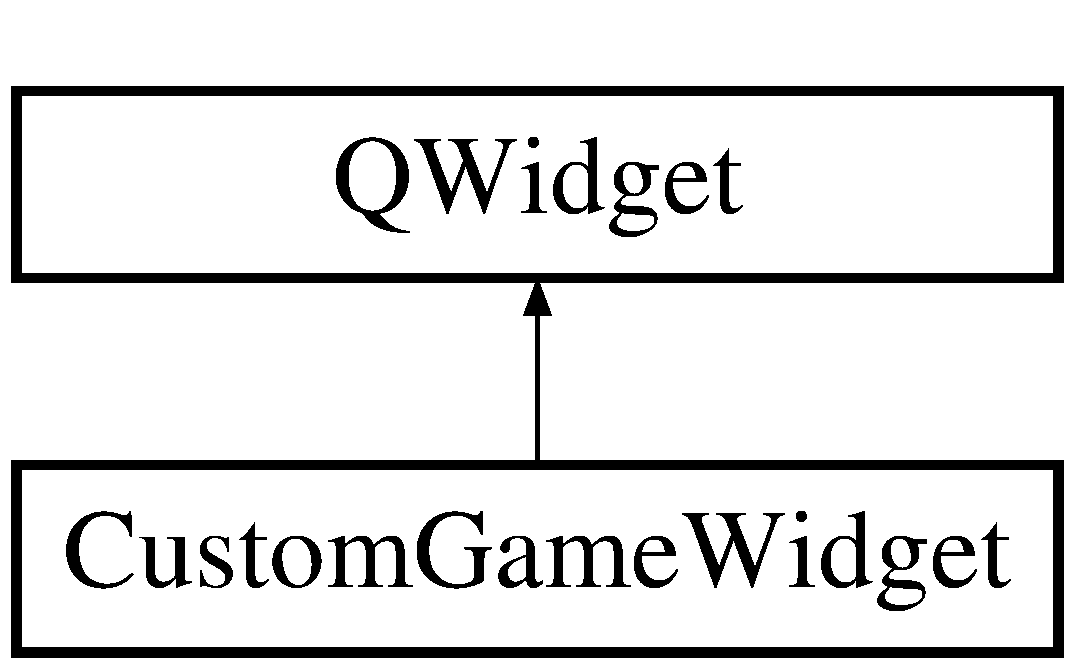
\includegraphics[height=2.000000cm]{class_custom_game_widget}
\end{center}
\end{figure}
\subsection*{Public Member Functions}
\begin{DoxyCompactItemize}
\item 
\hyperlink{class_custom_game_widget_a1c85b1e714a238a7afbcbb8dfa28f0b1}{Custom\+Game\+Widget} (Q\+Widget $\ast$parent=0)
\begin{DoxyCompactList}\small\item\em \hyperlink{class_custom_game_widget}{Custom\+Game\+Widget} Constructor. \end{DoxyCompactList}\item 
\mbox{\Hypertarget{class_custom_game_widget_a43b0436fa948b2b44009fe2e656ac3e0}\label{class_custom_game_widget_a43b0436fa948b2b44009fe2e656ac3e0}} 
\hyperlink{class_custom_game_widget_a43b0436fa948b2b44009fe2e656ac3e0}{$\sim$\+Custom\+Game\+Widget} ()
\begin{DoxyCompactList}\small\item\em Destructor. \end{DoxyCompactList}\item 
\mbox{\Hypertarget{class_custom_game_widget_aa9e4d0f12c9070a0e432631754f8913a}\label{class_custom_game_widget_aa9e4d0f12c9070a0e432631754f8913a}} 
void \hyperlink{class_custom_game_widget_aa9e4d0f12c9070a0e432631754f8913a}{reset\+\_\+buttons} ()
\begin{DoxyCompactList}\small\item\em reset\+\_\+buttons Reset the buttons of the board (style,enable etc..). \end{DoxyCompactList}\item 
void \hyperlink{class_custom_game_widget_abd589dcb5502f401773de7f1d349954a}{enable\+\_\+buttons} (bool enable)
\begin{DoxyCompactList}\small\item\em enable\+\_\+buttons Enable the buttons or not (play buttons). \end{DoxyCompactList}\item 
void \hyperlink{class_custom_game_widget_ae34e750a94a537ee435aa31311b5f495}{set\+\_\+button\+\_\+value} (class Q\+Push\+Button $\ast$button, int value)
\begin{DoxyCompactList}\small\item\em set\+\_\+button\+\_\+value Set the button value, Either cross or circle depending on who played. \end{DoxyCompactList}\end{DoxyCompactItemize}


\subsection{Detailed Description}
The \hyperlink{class_custom_game_widget}{Custom\+Game\+Widget} class Widget used to handle the game board. 

\subsection{Constructor \& Destructor Documentation}
\mbox{\Hypertarget{class_custom_game_widget_a1c85b1e714a238a7afbcbb8dfa28f0b1}\label{class_custom_game_widget_a1c85b1e714a238a7afbcbb8dfa28f0b1}} 
\index{Custom\+Game\+Widget@{Custom\+Game\+Widget}!Custom\+Game\+Widget@{Custom\+Game\+Widget}}
\index{Custom\+Game\+Widget@{Custom\+Game\+Widget}!Custom\+Game\+Widget@{Custom\+Game\+Widget}}
\subsubsection{\texorpdfstring{Custom\+Game\+Widget()}{CustomGameWidget()}}
{\footnotesize\ttfamily Custom\+Game\+Widget\+::\+Custom\+Game\+Widget (\begin{DoxyParamCaption}\item[{Q\+Widget $\ast$}]{parent = {\ttfamily 0} }\end{DoxyParamCaption})\hspace{0.3cm}{\ttfamily [explicit]}}



\hyperlink{class_custom_game_widget}{Custom\+Game\+Widget} Constructor. 


\begin{DoxyParams}{Parameters}
{\em parent} & Parent widget, default is null. \\
\hline
\end{DoxyParams}


\subsection{Member Function Documentation}
\mbox{\Hypertarget{class_custom_game_widget_abd589dcb5502f401773de7f1d349954a}\label{class_custom_game_widget_abd589dcb5502f401773de7f1d349954a}} 
\index{Custom\+Game\+Widget@{Custom\+Game\+Widget}!enable\+\_\+buttons@{enable\+\_\+buttons}}
\index{enable\+\_\+buttons@{enable\+\_\+buttons}!Custom\+Game\+Widget@{Custom\+Game\+Widget}}
\subsubsection{\texorpdfstring{enable\+\_\+buttons()}{enable\_buttons()}}
{\footnotesize\ttfamily void Custom\+Game\+Widget\+::enable\+\_\+buttons (\begin{DoxyParamCaption}\item[{bool}]{enable }\end{DoxyParamCaption})}



enable\+\_\+buttons Enable the buttons or not (play buttons). 


\begin{DoxyParams}{Parameters}
{\em enable} & If true, will enable the buttons. \\
\hline
\end{DoxyParams}
\mbox{\Hypertarget{class_custom_game_widget_ae34e750a94a537ee435aa31311b5f495}\label{class_custom_game_widget_ae34e750a94a537ee435aa31311b5f495}} 
\index{Custom\+Game\+Widget@{Custom\+Game\+Widget}!set\+\_\+button\+\_\+value@{set\+\_\+button\+\_\+value}}
\index{set\+\_\+button\+\_\+value@{set\+\_\+button\+\_\+value}!Custom\+Game\+Widget@{Custom\+Game\+Widget}}
\subsubsection{\texorpdfstring{set\+\_\+button\+\_\+value()}{set\_button\_value()}}
{\footnotesize\ttfamily void Custom\+Game\+Widget\+::set\+\_\+button\+\_\+value (\begin{DoxyParamCaption}\item[{class Q\+Push\+Button $\ast$}]{button,  }\item[{int}]{value }\end{DoxyParamCaption})}



set\+\_\+button\+\_\+value Set the button value, Either cross or circle depending on who played. 


\begin{DoxyParams}{Parameters}
{\em button} & Pointer to the button to be edited \\
\hline
{\em value} & Value of the symbol of the player that pressed the button. \\
\hline
\end{DoxyParams}


The documentation for this class was generated from the following files\+:\begin{DoxyCompactItemize}
\item 
Widget/customgamewidget.\+h\item 
Widget/customgamewidget.\+cpp\end{DoxyCompactItemize}

\hypertarget{class_game_window}{}\section{Game\+Window Class Reference}
\label{class_game_window}\index{Game\+Window@{Game\+Window}}


The \hyperlink{class_game_window}{Game\+Window} class The game window class responsible of displaying the game.  




{\ttfamily \#include $<$Game\+Window.\+h$>$}

Inheritance diagram for Game\+Window\+:\begin{figure}[H]
\begin{center}
\leavevmode
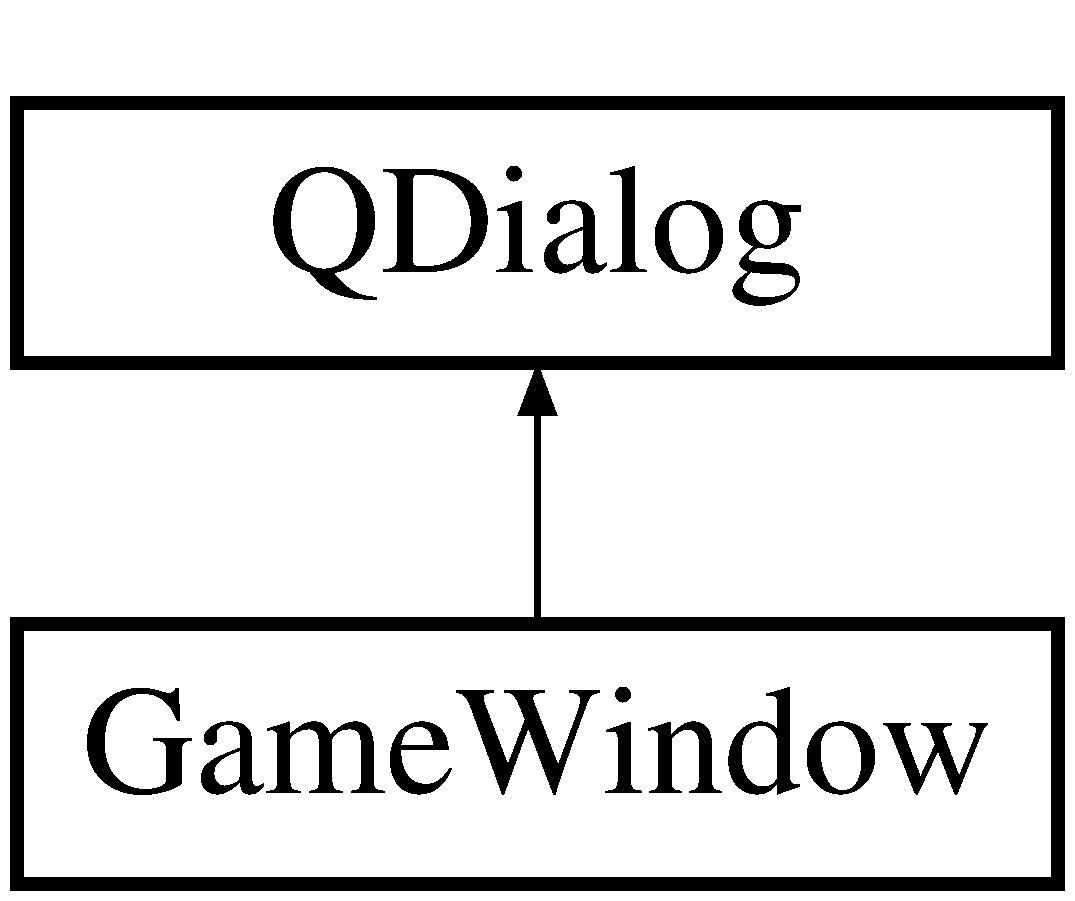
\includegraphics[height=2.000000cm]{class_game_window}
\end{center}
\end{figure}
\subsection*{Public Member Functions}
\begin{DoxyCompactItemize}
\item 
\hyperlink{class_game_window_a016b254d770fc4c2ce4a21a4c6f38fbc}{Game\+Window} (Q\+Widget $\ast$parent=0)
\begin{DoxyCompactList}\small\item\em \hyperlink{class_game_window}{Game\+Window} Constructor. \end{DoxyCompactList}\item 
\mbox{\Hypertarget{class_game_window_a55b071c0390e45c064a160c1e6baaa08}\label{class_game_window_a55b071c0390e45c064a160c1e6baaa08}} 
\hyperlink{class_game_window_a55b071c0390e45c064a160c1e6baaa08}{$\sim$\+Game\+Window} ()
\begin{DoxyCompactList}\small\item\em Destructor. \end{DoxyCompactList}\item 
void \hyperlink{class_game_window_a87e5f249822ac1bd895ad9bcd26a80af}{init\+\_\+ui} (Q\+String fpname, Q\+String spname, Q\+String current\+Player\+Name)
\begin{DoxyCompactList}\small\item\em init\+\_\+ui Initialize the ui. \end{DoxyCompactList}\item 
void \hyperlink{class_game_window_a6cb8a429ac545c93457ad00bd0242af3}{update\+\_\+scores\+\_\+ui} (Q\+String fpscore, Q\+String spscore)
\begin{DoxyCompactList}\small\item\em update\+\_\+scores\+\_\+ui Update the score from the different player \end{DoxyCompactList}\item 
void \hyperlink{class_game_window_a97c9a250fd9010a1ee4b39fef5325af7}{update\+\_\+current\+\_\+player\+\_\+name\+\_\+ui} (Q\+String name)
\begin{DoxyCompactList}\small\item\em update\+\_\+current\+\_\+player\+\_\+name\+\_\+ui Update the current player labe. \end{DoxyCompactList}\item 
void \hyperlink{class_game_window_adfdbef2f1c76091d1a14a07660baeb7f}{show\+\_\+winner} (bool show, Q\+String name=\char`\"{}\char`\"{})
\begin{DoxyCompactList}\small\item\em show\+\_\+winner Will display who is the winner as well as replay button to restart a new game. \end{DoxyCompactList}\item 
\mbox{\Hypertarget{class_game_window_a4b226699ff95a77a540f4d141f5cae4f}\label{class_game_window_a4b226699ff95a77a540f4d141f5cae4f}} 
void \hyperlink{class_game_window_a4b226699ff95a77a540f4d141f5cae4f}{reset\+\_\+game\+\_\+buttons} ()
\begin{DoxyCompactList}\small\item\em reset\+\_\+game\+\_\+buttons Reset the button of the game (style, enable, etc..) \end{DoxyCompactList}\item 
void \hyperlink{class_game_window_a55e1796bc70513802f85f3830140011b}{enable\+\_\+game\+\_\+buttons} (bool enable)
\begin{DoxyCompactList}\small\item\em enable\+\_\+game\+\_\+buttons Enable or not the button to be re usable. \end{DoxyCompactList}\item 
void \hyperlink{class_game_window_adb7764f6b74f57ba2197cb9f5a65c47b}{set\+\_\+button\+\_\+value} (Q\+Push\+Button $\ast$button, int value)
\begin{DoxyCompactList}\small\item\em set\+\_\+button\+\_\+value Set the current button value (if it is a cross or circle). \end{DoxyCompactList}\end{DoxyCompactItemize}


\subsection{Detailed Description}
The \hyperlink{class_game_window}{Game\+Window} class The game window class responsible of displaying the game. 

\subsection{Constructor \& Destructor Documentation}
\mbox{\Hypertarget{class_game_window_a016b254d770fc4c2ce4a21a4c6f38fbc}\label{class_game_window_a016b254d770fc4c2ce4a21a4c6f38fbc}} 
\index{Game\+Window@{Game\+Window}!Game\+Window@{Game\+Window}}
\index{Game\+Window@{Game\+Window}!Game\+Window@{Game\+Window}}
\subsubsection{\texorpdfstring{Game\+Window()}{GameWindow()}}
{\footnotesize\ttfamily Game\+Window\+::\+Game\+Window (\begin{DoxyParamCaption}\item[{Q\+Widget $\ast$}]{parent = {\ttfamily 0} }\end{DoxyParamCaption})\hspace{0.3cm}{\ttfamily [explicit]}}



\hyperlink{class_game_window}{Game\+Window} Constructor. 


\begin{DoxyParams}{Parameters}
{\em parent} & Parent widget of the window, default is null. \\
\hline
\end{DoxyParams}


\subsection{Member Function Documentation}
\mbox{\Hypertarget{class_game_window_a55e1796bc70513802f85f3830140011b}\label{class_game_window_a55e1796bc70513802f85f3830140011b}} 
\index{Game\+Window@{Game\+Window}!enable\+\_\+game\+\_\+buttons@{enable\+\_\+game\+\_\+buttons}}
\index{enable\+\_\+game\+\_\+buttons@{enable\+\_\+game\+\_\+buttons}!Game\+Window@{Game\+Window}}
\subsubsection{\texorpdfstring{enable\+\_\+game\+\_\+buttons()}{enable\_game\_buttons()}}
{\footnotesize\ttfamily void Game\+Window\+::enable\+\_\+game\+\_\+buttons (\begin{DoxyParamCaption}\item[{bool}]{enable }\end{DoxyParamCaption})}



enable\+\_\+game\+\_\+buttons Enable or not the button to be re usable. 


\begin{DoxyParams}{Parameters}
{\em enable} & True will enable the buttons. \\
\hline
\end{DoxyParams}
\mbox{\Hypertarget{class_game_window_a87e5f249822ac1bd895ad9bcd26a80af}\label{class_game_window_a87e5f249822ac1bd895ad9bcd26a80af}} 
\index{Game\+Window@{Game\+Window}!init\+\_\+ui@{init\+\_\+ui}}
\index{init\+\_\+ui@{init\+\_\+ui}!Game\+Window@{Game\+Window}}
\subsubsection{\texorpdfstring{init\+\_\+ui()}{init\_ui()}}
{\footnotesize\ttfamily void Game\+Window\+::init\+\_\+ui (\begin{DoxyParamCaption}\item[{Q\+String}]{fpname,  }\item[{Q\+String}]{spname,  }\item[{Q\+String}]{current\+Player\+Name }\end{DoxyParamCaption})}



init\+\_\+ui Initialize the ui. 


\begin{DoxyParams}{Parameters}
{\em fpname} & First Player Name. \\
\hline
{\em spname} & Second Player Name. \\
\hline
{\em current\+Player\+Name} & Current Player name. \\
\hline
\end{DoxyParams}
\mbox{\Hypertarget{class_game_window_adb7764f6b74f57ba2197cb9f5a65c47b}\label{class_game_window_adb7764f6b74f57ba2197cb9f5a65c47b}} 
\index{Game\+Window@{Game\+Window}!set\+\_\+button\+\_\+value@{set\+\_\+button\+\_\+value}}
\index{set\+\_\+button\+\_\+value@{set\+\_\+button\+\_\+value}!Game\+Window@{Game\+Window}}
\subsubsection{\texorpdfstring{set\+\_\+button\+\_\+value()}{set\_button\_value()}}
{\footnotesize\ttfamily void Game\+Window\+::set\+\_\+button\+\_\+value (\begin{DoxyParamCaption}\item[{Q\+Push\+Button $\ast$}]{button,  }\item[{int}]{value }\end{DoxyParamCaption})}



set\+\_\+button\+\_\+value Set the current button value (if it is a cross or circle). 


\begin{DoxyParams}{Parameters}
{\em button} & Button pointer to be set. \\
\hline
{\em value} & New value of the button. \\
\hline
\end{DoxyParams}
\mbox{\Hypertarget{class_game_window_adfdbef2f1c76091d1a14a07660baeb7f}\label{class_game_window_adfdbef2f1c76091d1a14a07660baeb7f}} 
\index{Game\+Window@{Game\+Window}!show\+\_\+winner@{show\+\_\+winner}}
\index{show\+\_\+winner@{show\+\_\+winner}!Game\+Window@{Game\+Window}}
\subsubsection{\texorpdfstring{show\+\_\+winner()}{show\_winner()}}
{\footnotesize\ttfamily void Game\+Window\+::show\+\_\+winner (\begin{DoxyParamCaption}\item[{bool}]{show,  }\item[{Q\+String}]{name = {\ttfamily \char`\"{}\char`\"{}} }\end{DoxyParamCaption})}



show\+\_\+winner Will display who is the winner as well as replay button to restart a new game. 


\begin{DoxyParams}{Parameters}
{\em show} & True if we should show the winner. \\
\hline
{\em name} & Name of the winner. \\
\hline
\end{DoxyParams}
\mbox{\Hypertarget{class_game_window_a97c9a250fd9010a1ee4b39fef5325af7}\label{class_game_window_a97c9a250fd9010a1ee4b39fef5325af7}} 
\index{Game\+Window@{Game\+Window}!update\+\_\+current\+\_\+player\+\_\+name\+\_\+ui@{update\+\_\+current\+\_\+player\+\_\+name\+\_\+ui}}
\index{update\+\_\+current\+\_\+player\+\_\+name\+\_\+ui@{update\+\_\+current\+\_\+player\+\_\+name\+\_\+ui}!Game\+Window@{Game\+Window}}
\subsubsection{\texorpdfstring{update\+\_\+current\+\_\+player\+\_\+name\+\_\+ui()}{update\_current\_player\_name\_ui()}}
{\footnotesize\ttfamily void Game\+Window\+::update\+\_\+current\+\_\+player\+\_\+name\+\_\+ui (\begin{DoxyParamCaption}\item[{Q\+String}]{name }\end{DoxyParamCaption})}



update\+\_\+current\+\_\+player\+\_\+name\+\_\+ui Update the current player labe. 


\begin{DoxyParams}{Parameters}
{\em name} & Name of the current player. \\
\hline
\end{DoxyParams}
\mbox{\Hypertarget{class_game_window_a6cb8a429ac545c93457ad00bd0242af3}\label{class_game_window_a6cb8a429ac545c93457ad00bd0242af3}} 
\index{Game\+Window@{Game\+Window}!update\+\_\+scores\+\_\+ui@{update\+\_\+scores\+\_\+ui}}
\index{update\+\_\+scores\+\_\+ui@{update\+\_\+scores\+\_\+ui}!Game\+Window@{Game\+Window}}
\subsubsection{\texorpdfstring{update\+\_\+scores\+\_\+ui()}{update\_scores\_ui()}}
{\footnotesize\ttfamily void Game\+Window\+::update\+\_\+scores\+\_\+ui (\begin{DoxyParamCaption}\item[{Q\+String}]{fpscore,  }\item[{Q\+String}]{spscore }\end{DoxyParamCaption})}



update\+\_\+scores\+\_\+ui Update the score from the different player 


\begin{DoxyParams}{Parameters}
{\em fpscore} & First player score. \\
\hline
{\em spscore} & Second player score. \\
\hline
\end{DoxyParams}


The documentation for this class was generated from the following files\+:\begin{DoxyCompactItemize}
\item 
Game\+Window.\+h\item 
Game\+Window.\+cpp\end{DoxyCompactItemize}

\hypertarget{class_i_board}{}\section{I\+Board Class Reference}
\label{class_i_board}\index{I\+Board@{I\+Board}}


The \hyperlink{class_i_board}{I\+Board} class interface is used as a template to create boards for board games.  




{\ttfamily \#include $<$I\+Board.\+h$>$}

Inheritance diagram for I\+Board\+:\begin{figure}[H]
\begin{center}
\leavevmode
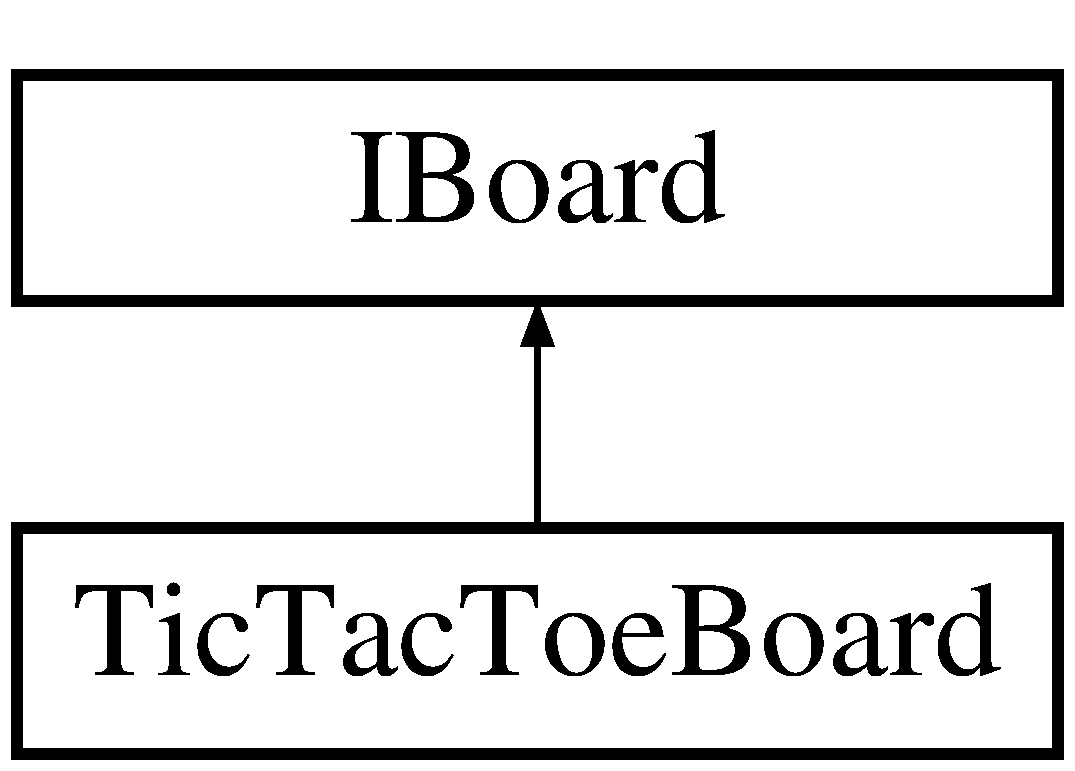
\includegraphics[height=2.000000cm]{class_i_board}
\end{center}
\end{figure}
\subsection*{Public Member Functions}
\begin{DoxyCompactItemize}
\item 
\mbox{\Hypertarget{class_i_board_afb18c7820f9051616ca6f7e6cddad4a8}\label{class_i_board_afb18c7820f9051616ca6f7e6cddad4a8}} 
virtual void \hyperlink{class_i_board_afb18c7820f9051616ca6f7e6cddad4a8}{init} ()=0
\begin{DoxyCompactList}\small\item\em pure virtual method used to template initialization of the game board. \end{DoxyCompactList}\item 
\mbox{\Hypertarget{class_i_board_acefb3aefbb5e612b2f7eefa52dc04e62}\label{class_i_board_acefb3aefbb5e612b2f7eefa52dc04e62}} 
virtual void \hyperlink{class_i_board_acefb3aefbb5e612b2f7eefa52dc04e62}{reset} ()=0
\begin{DoxyCompactList}\small\item\em pure virtal method used to template the reset the game board method(cases, pawns, values etc..). \end{DoxyCompactList}\end{DoxyCompactItemize}


\subsection{Detailed Description}
The \hyperlink{class_i_board}{I\+Board} class interface is used as a template to create boards for board games. 

The documentation for this class was generated from the following file\+:\begin{DoxyCompactItemize}
\item 
Board/I\+Board.\+h\end{DoxyCompactItemize}

\hypertarget{class_i_game_manager}{}\section{I\+Game\+Manager Class Reference}
\label{class_i_game_manager}\index{I\+Game\+Manager@{I\+Game\+Manager}}


The \hyperlink{class_i_game_manager}{I\+Game\+Manager} class Interface created to implement a Game\+Manager.  




{\ttfamily \#include $<$I\+Game\+Manager.\+h$>$}

Inheritance diagram for I\+Game\+Manager\+:\begin{figure}[H]
\begin{center}
\leavevmode
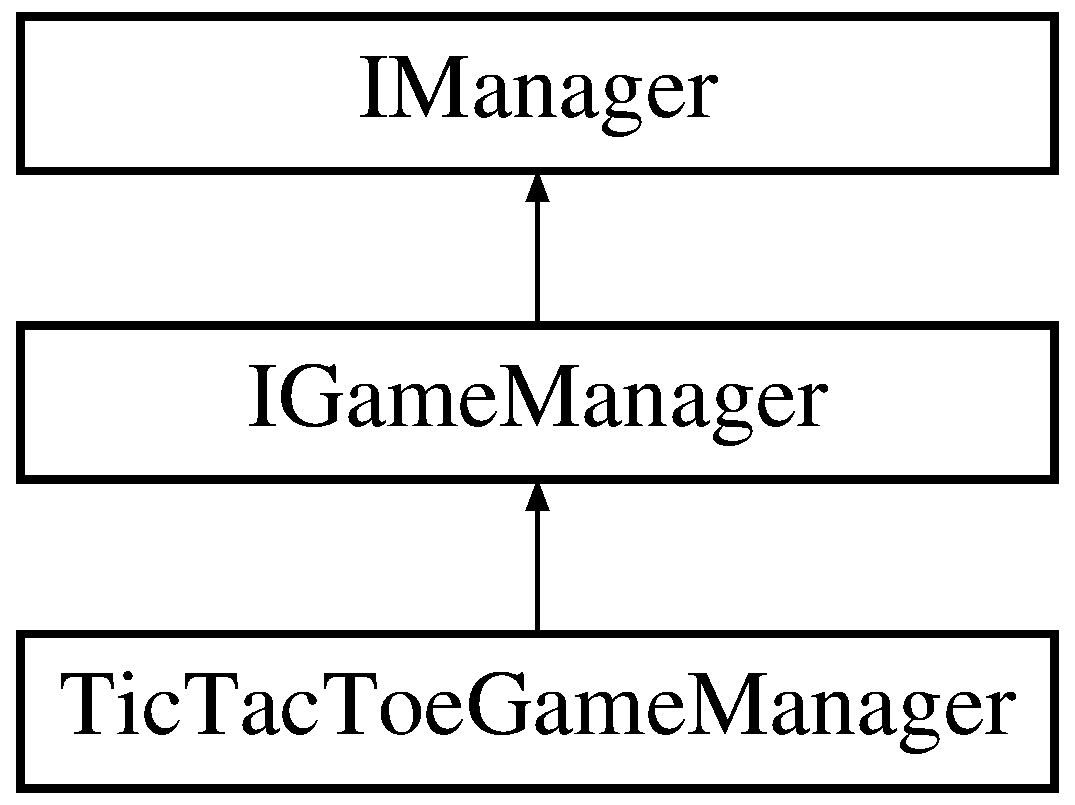
\includegraphics[height=3.000000cm]{class_i_game_manager}
\end{center}
\end{figure}
\subsection*{Public Member Functions}
\begin{DoxyCompactItemize}
\item 
\mbox{\Hypertarget{class_i_game_manager_a355e2344fc289700bfa0aab3ba32d1e8}\label{class_i_game_manager_a355e2344fc289700bfa0aab3ba32d1e8}} 
virtual void \hyperlink{class_i_game_manager_a355e2344fc289700bfa0aab3ba32d1e8}{init} ()=0
\begin{DoxyCompactList}\small\item\em init Initialize the interface \end{DoxyCompactList}\item 
virtual void \hyperlink{class_i_game_manager_a197ed85a1deadeb414b3030e11d0bf1e}{create\+\_\+player} (const std\+::string \&name, const int \&symbol)=0
\begin{DoxyCompactList}\small\item\em create\+\_\+player Create a player and will store it in a container. \end{DoxyCompactList}\end{DoxyCompactItemize}


\subsection{Detailed Description}
The \hyperlink{class_i_game_manager}{I\+Game\+Manager} class Interface created to implement a Game\+Manager. 

\subsection{Member Function Documentation}
\mbox{\Hypertarget{class_i_game_manager_a197ed85a1deadeb414b3030e11d0bf1e}\label{class_i_game_manager_a197ed85a1deadeb414b3030e11d0bf1e}} 
\index{I\+Game\+Manager@{I\+Game\+Manager}!create\+\_\+player@{create\+\_\+player}}
\index{create\+\_\+player@{create\+\_\+player}!I\+Game\+Manager@{I\+Game\+Manager}}
\subsubsection{\texorpdfstring{create\+\_\+player()}{create\_player()}}
{\footnotesize\ttfamily virtual void I\+Game\+Manager\+::create\+\_\+player (\begin{DoxyParamCaption}\item[{const std\+::string \&}]{name,  }\item[{const int \&}]{symbol }\end{DoxyParamCaption})\hspace{0.3cm}{\ttfamily [pure virtual]}}



create\+\_\+player Create a player and will store it in a container. 


\begin{DoxyParams}{Parameters}
{\em name} & Name of the player. \\
\hline
{\em symbol} & Symbol / value used by the player to set a case in the board. \\
\hline
\end{DoxyParams}


Implemented in \hyperlink{class_tic_tac_toe_game_manager_a2d2b1cf7c29f760811f3ecc983dd2c5f}{Tic\+Tac\+Toe\+Game\+Manager}.



The documentation for this class was generated from the following file\+:\begin{DoxyCompactItemize}
\item 
Manager/I\+Game\+Manager.\+h\end{DoxyCompactItemize}

\hypertarget{class_i_manager}{}\section{I\+Manager Class Reference}
\label{class_i_manager}\index{I\+Manager@{I\+Manager}}


The \hyperlink{class_i_manager}{I\+Manager} class Base interface class to template a manager object. Manager object should be responsible of handling actions between data and ui.  




{\ttfamily \#include $<$I\+Manager.\+h$>$}

Inheritance diagram for I\+Manager\+:\begin{figure}[H]
\begin{center}
\leavevmode
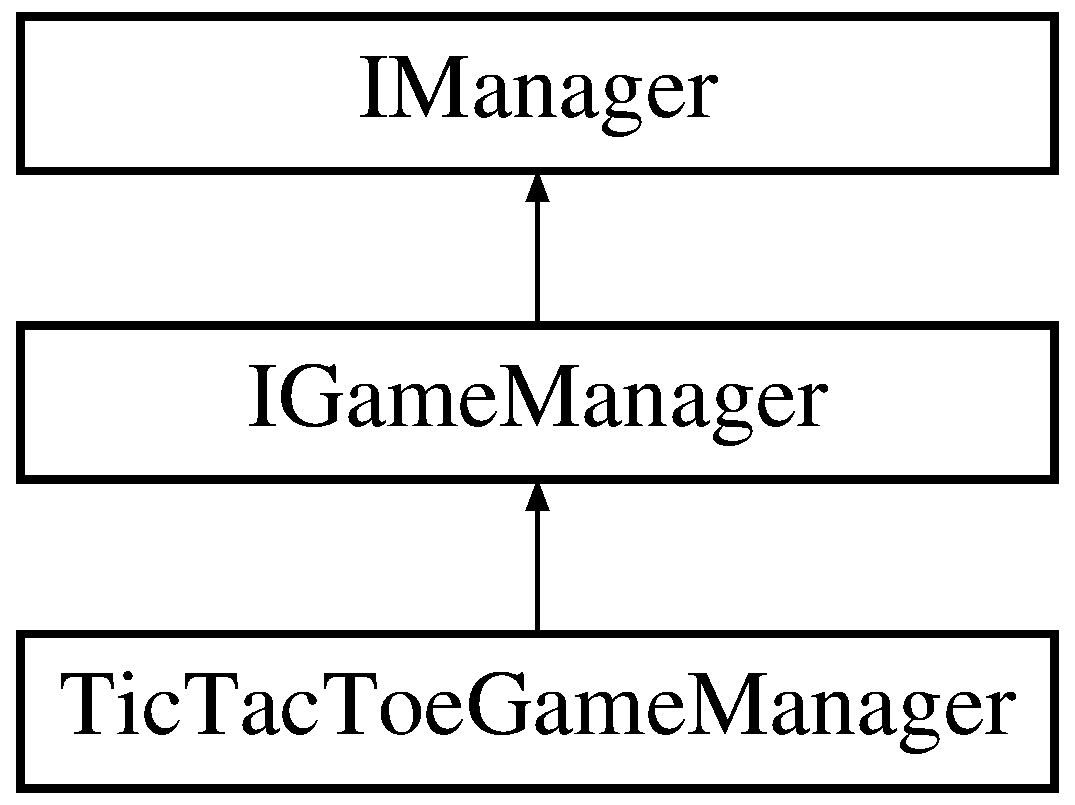
\includegraphics[height=3.000000cm]{class_i_manager}
\end{center}
\end{figure}
\subsection*{Public Member Functions}
\begin{DoxyCompactItemize}
\item 
\mbox{\Hypertarget{class_i_manager_ae8b36e4b4178abc62b84bcf20a63aa5b}\label{class_i_manager_ae8b36e4b4178abc62b84bcf20a63aa5b}} 
virtual void \hyperlink{class_i_manager_ae8b36e4b4178abc62b84bcf20a63aa5b}{init} ()=0
\begin{DoxyCompactList}\small\item\em init Initialize the interface. \end{DoxyCompactList}\end{DoxyCompactItemize}


\subsection{Detailed Description}
The \hyperlink{class_i_manager}{I\+Manager} class Base interface class to template a manager object. Manager object should be responsible of handling actions between data and ui. 

The documentation for this class was generated from the following file\+:\begin{DoxyCompactItemize}
\item 
Manager/I\+Manager.\+h\end{DoxyCompactItemize}

\hypertarget{class_i_player}{}\section{I\+Player Class Reference}
\label{class_i_player}\index{I\+Player@{I\+Player}}


The \hyperlink{class_i_player}{I\+Player} interface used as a template to implement players.  




{\ttfamily \#include $<$I\+Player.\+h$>$}

Inheritance diagram for I\+Player\+:\begin{figure}[H]
\begin{center}
\leavevmode
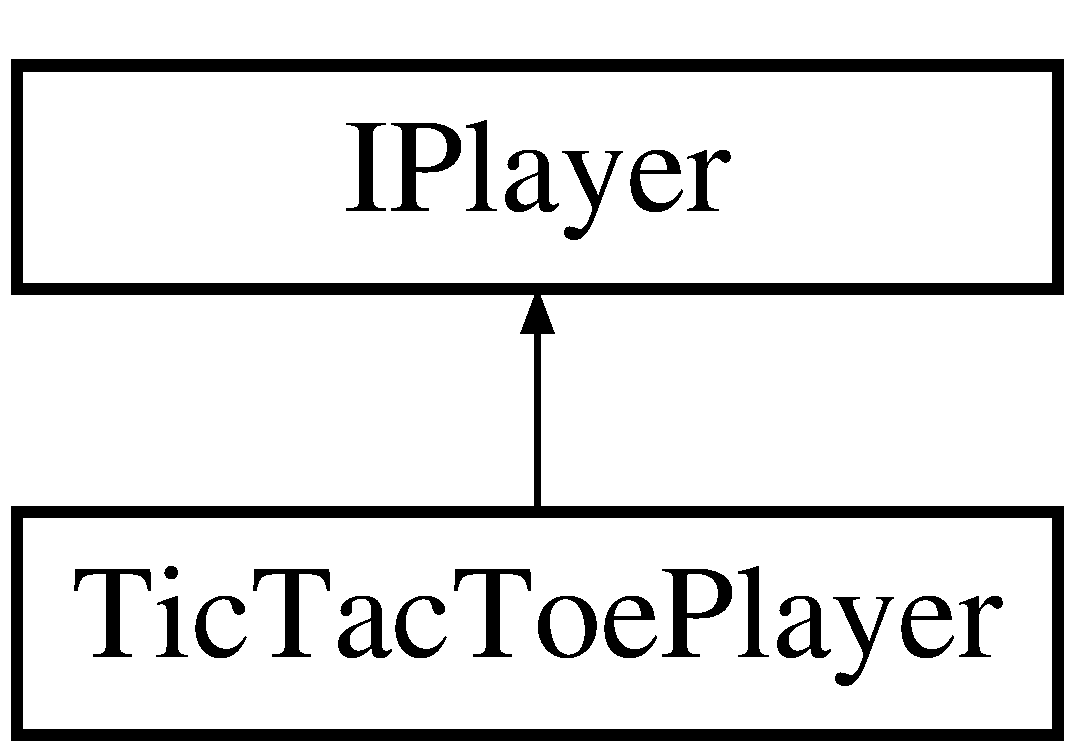
\includegraphics[height=2.000000cm]{class_i_player}
\end{center}
\end{figure}
\subsection*{Public Member Functions}
\begin{DoxyCompactItemize}
\item 
\mbox{\Hypertarget{class_i_player_a55ac140b5f98671b06a0ca51bd0314a1}\label{class_i_player_a55ac140b5f98671b06a0ca51bd0314a1}} 
virtual std\+::string {\bfseries get\+\_\+name} () const =0
\item 
\mbox{\Hypertarget{class_i_player_a3c21c9e94e3828adf3a78fe057b22f38}\label{class_i_player_a3c21c9e94e3828adf3a78fe057b22f38}} 
virtual void {\bfseries set\+\_\+name} (const std\+::string \&name)=0
\item 
\mbox{\Hypertarget{class_i_player_aed92c551c7a7a757ecafbc7b70cd88cf}\label{class_i_player_aed92c551c7a7a757ecafbc7b70cd88cf}} 
virtual int {\bfseries get\+\_\+score} () const =0
\item 
\mbox{\Hypertarget{class_i_player_ad8858145f3d117c7615589f40e6def23}\label{class_i_player_ad8858145f3d117c7615589f40e6def23}} 
virtual void {\bfseries update\+\_\+score} ()=0
\item 
\mbox{\Hypertarget{class_i_player_a3dc4f830accf157f1fe84c0736f05e7f}\label{class_i_player_a3dc4f830accf157f1fe84c0736f05e7f}} 
virtual void {\bfseries reset\+\_\+score} ()=0
\item 
\mbox{\Hypertarget{class_i_player_a16753695f90625ac8fe7538f620525df}\label{class_i_player_a16753695f90625ac8fe7538f620525df}} 
virtual int {\bfseries get\+\_\+symbol} () const =0
\end{DoxyCompactItemize}


\subsection{Detailed Description}
The \hyperlink{class_i_player}{I\+Player} interface used as a template to implement players. 

The documentation for this class was generated from the following file\+:\begin{DoxyCompactItemize}
\item 
Player/I\+Player.\+h\end{DoxyCompactItemize}

\hypertarget{class_i_score}{}\section{I\+Score Class Reference}
\label{class_i_score}\index{I\+Score@{I\+Score}}


The \hyperlink{class_i_score}{I\+Score} class Interface used to template what a score will be.  




{\ttfamily \#include $<$I\+Score.\+h$>$}

Inheritance diagram for I\+Score\+:\begin{figure}[H]
\begin{center}
\leavevmode
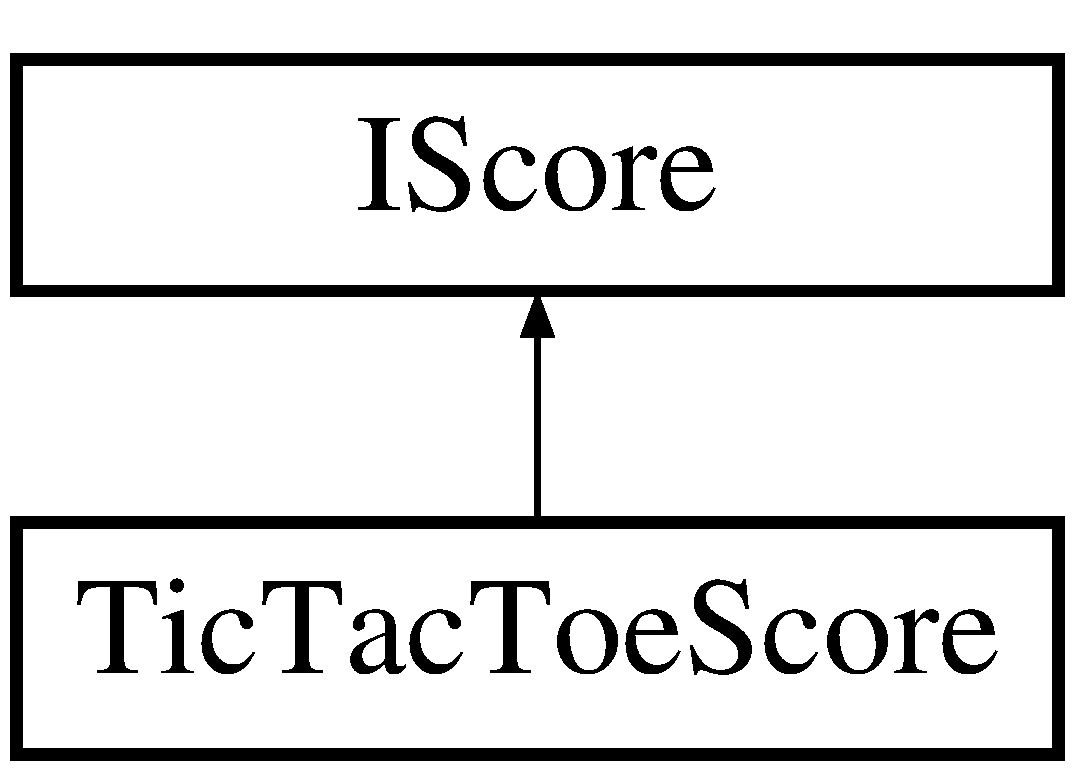
\includegraphics[height=2.000000cm]{class_i_score}
\end{center}
\end{figure}
\subsection*{Public Member Functions}
\begin{DoxyCompactItemize}
\item 
\mbox{\Hypertarget{class_i_score_a89f89e87a6442b5de524dc13248fc39f}\label{class_i_score_a89f89e87a6442b5de524dc13248fc39f}} 
virtual void {\bfseries init} ()=0
\item 
\mbox{\Hypertarget{class_i_score_a80c52a4d42d18dee5d32b1de587dab33}\label{class_i_score_a80c52a4d42d18dee5d32b1de587dab33}} 
virtual void {\bfseries update} ()=0
\item 
\mbox{\Hypertarget{class_i_score_aec3d808d09c6bd5ba89ee7ae8166eece}\label{class_i_score_aec3d808d09c6bd5ba89ee7ae8166eece}} 
virtual void {\bfseries reset} ()=0
\item 
\mbox{\Hypertarget{class_i_score_aa47f3fc1c4448f09acfbbee021680e08}\label{class_i_score_aa47f3fc1c4448f09acfbbee021680e08}} 
virtual int {\bfseries get} () const =0
\end{DoxyCompactItemize}


\subsection{Detailed Description}
The \hyperlink{class_i_score}{I\+Score} class Interface used to template what a score will be. 

The documentation for this class was generated from the following file\+:\begin{DoxyCompactItemize}
\item 
Score/I\+Score.\+h\end{DoxyCompactItemize}

\hypertarget{class_main_window}{}\section{Main\+Window Class Reference}
\label{class_main_window}\index{Main\+Window@{Main\+Window}}


The \hyperlink{class_main_window}{Main\+Window} class First window to setup the name and rule of the tic tac toe.  




{\ttfamily \#include $<$mainwindow.\+h$>$}

Inheritance diagram for Main\+Window\+:\begin{figure}[H]
\begin{center}
\leavevmode
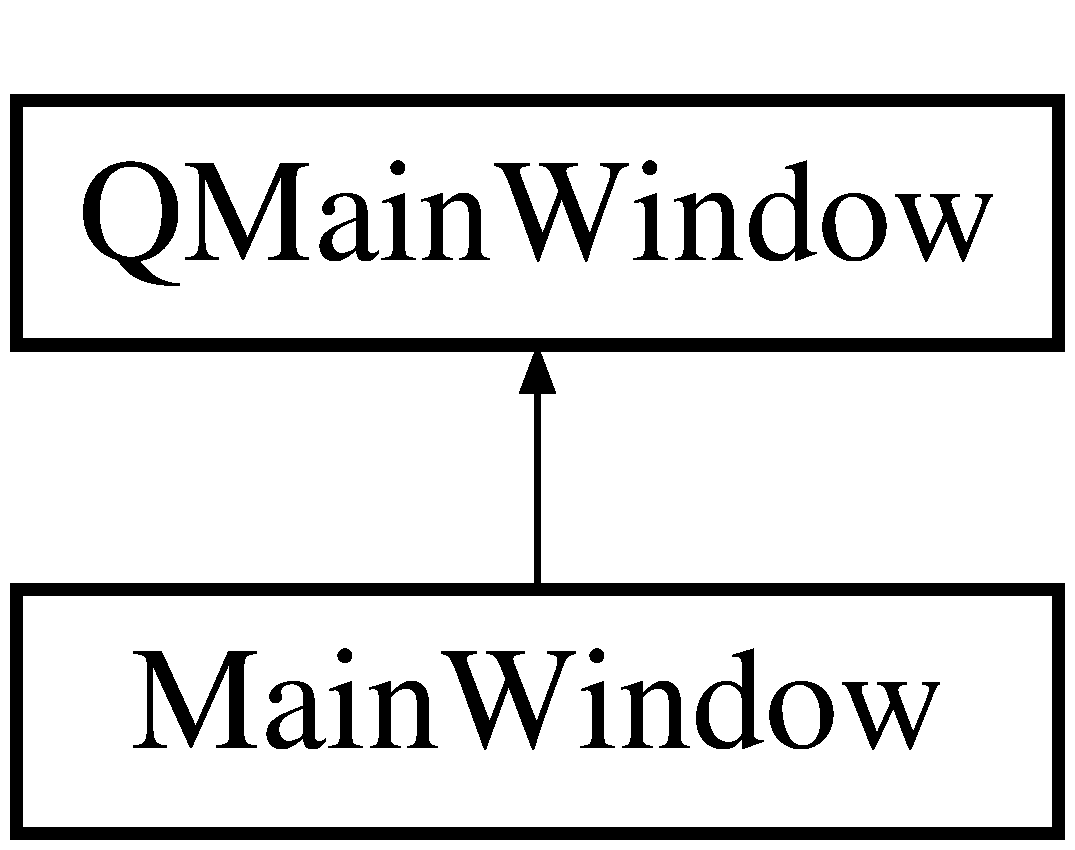
\includegraphics[height=2.000000cm]{class_main_window}
\end{center}
\end{figure}
\subsection*{Public Member Functions}
\begin{DoxyCompactItemize}
\item 
\hyperlink{class_main_window_a8b244be8b7b7db1b08de2a2acb9409db}{Main\+Window} (Q\+Widget $\ast$parent=0)
\begin{DoxyCompactList}\small\item\em \hyperlink{class_main_window}{Main\+Window} Constructor. \end{DoxyCompactList}\item 
\mbox{\Hypertarget{class_main_window_ae98d00a93bc118200eeef9f9bba1dba7}\label{class_main_window_ae98d00a93bc118200eeef9f9bba1dba7}} 
\hyperlink{class_main_window_ae98d00a93bc118200eeef9f9bba1dba7}{$\sim$\+Main\+Window} ()
\begin{DoxyCompactList}\small\item\em Destructor. \end{DoxyCompactList}\item 
\mbox{\Hypertarget{class_main_window_a422173d1931306612cdca9aba1d57507}\label{class_main_window_a422173d1931306612cdca9aba1d57507}} 
void \hyperlink{class_main_window_a422173d1931306612cdca9aba1d57507}{create\+\_\+game\+\_\+window} ()
\begin{DoxyCompactList}\small\item\em create\+\_\+game\+\_\+window Create the game window. \end{DoxyCompactList}\end{DoxyCompactItemize}


\subsection{Detailed Description}
The \hyperlink{class_main_window}{Main\+Window} class First window to setup the name and rule of the tic tac toe. 

\subsection{Constructor \& Destructor Documentation}
\mbox{\Hypertarget{class_main_window_a8b244be8b7b7db1b08de2a2acb9409db}\label{class_main_window_a8b244be8b7b7db1b08de2a2acb9409db}} 
\index{Main\+Window@{Main\+Window}!Main\+Window@{Main\+Window}}
\index{Main\+Window@{Main\+Window}!Main\+Window@{Main\+Window}}
\subsubsection{\texorpdfstring{Main\+Window()}{MainWindow()}}
{\footnotesize\ttfamily Main\+Window\+::\+Main\+Window (\begin{DoxyParamCaption}\item[{Q\+Widget $\ast$}]{parent = {\ttfamily 0} }\end{DoxyParamCaption})\hspace{0.3cm}{\ttfamily [explicit]}}



\hyperlink{class_main_window}{Main\+Window} Constructor. 


\begin{DoxyParams}{Parameters}
{\em parent} & Parent widget, default is null. \\
\hline
\end{DoxyParams}


The documentation for this class was generated from the following files\+:\begin{DoxyCompactItemize}
\item 
mainwindow.\+h\item 
mainwindow.\+cpp\end{DoxyCompactItemize}

\hypertarget{class_singleton}{}\section{Singleton$<$ T $>$ Class Template Reference}
\label{class_singleton}\index{Singleton$<$ T $>$@{Singleton$<$ T $>$}}


The \hyperlink{class_singleton}{Singleton} class.  




{\ttfamily \#include $<$Singleton.\+h$>$}

\subsection*{Static Public Member Functions}
\begin{DoxyCompactItemize}
\item 
static T $\ast$ \hyperlink{class_singleton_a653aa7351e551af1bae09d01aa713091}{instance} ()
\begin{DoxyCompactList}\small\item\em Instance \hyperlink{class_singleton}{Singleton} instance to have only one instance of the object. Call my\+Class\+::instance(). \end{DoxyCompactList}\item 
\mbox{\Hypertarget{class_singleton_a4e002a1eab6553b9bce6af8ebd4d3804}\label{class_singleton_a4e002a1eab6553b9bce6af8ebd4d3804}} 
static void \hyperlink{class_singleton_a4e002a1eab6553b9bce6af8ebd4d3804}{destroy} ()
\begin{DoxyCompactList}\small\item\em destroy Delete the current singelton. \end{DoxyCompactList}\end{DoxyCompactItemize}
\subsection*{Protected Member Functions}
\begin{DoxyCompactItemize}
\item 
\mbox{\Hypertarget{class_singleton_a923b995920da9c06590adb170ab2f890}\label{class_singleton_a923b995920da9c06590adb170ab2f890}} 
\hyperlink{class_singleton_a923b995920da9c06590adb170ab2f890}{Singleton} ()
\begin{DoxyCompactList}\small\item\em Default Constructor. \end{DoxyCompactList}\item 
\mbox{\Hypertarget{class_singleton_ac6e7af82cba33f561bd64e5e0243e7f8}\label{class_singleton_ac6e7af82cba33f561bd64e5e0243e7f8}} 
\hyperlink{class_singleton_ac6e7af82cba33f561bd64e5e0243e7f8}{$\sim$\+Singleton} ()
\begin{DoxyCompactList}\small\item\em Destructor. \end{DoxyCompactList}\end{DoxyCompactItemize}


\subsection{Detailed Description}
\subsubsection*{template$<$class T$>$\newline
class Singleton$<$ T $>$}

The \hyperlink{class_singleton}{Singleton} class. 

\subsection{Member Function Documentation}
\mbox{\Hypertarget{class_singleton_a653aa7351e551af1bae09d01aa713091}\label{class_singleton_a653aa7351e551af1bae09d01aa713091}} 
\index{Singleton@{Singleton}!instance@{instance}}
\index{instance@{instance}!Singleton@{Singleton}}
\subsubsection{\texorpdfstring{instance()}{instance()}}
{\footnotesize\ttfamily template$<$class T$>$ \\
static T$\ast$ \hyperlink{class_singleton}{Singleton}$<$ T $>$\+::instance (\begin{DoxyParamCaption}{ }\end{DoxyParamCaption})\hspace{0.3cm}{\ttfamily [inline]}, {\ttfamily [static]}}



Instance \hyperlink{class_singleton}{Singleton} instance to have only one instance of the object. Call my\+Class\+::instance(). 

\begin{DoxyReturn}{Returns}

\end{DoxyReturn}


The documentation for this class was generated from the following file\+:\begin{DoxyCompactItemize}
\item 
Misc/Singleton.\+h\end{DoxyCompactItemize}

\hypertarget{class_tic_tac_toe_board}{}\section{Tic\+Tac\+Toe\+Board Class Reference}
\label{class_tic_tac_toe_board}\index{Tic\+Tac\+Toe\+Board@{Tic\+Tac\+Toe\+Board}}


\hyperlink{class_tic_tac_toe_board}{Tic\+Tac\+Toe\+Board} class will be holding the values for each each case of the board on a 3x3 for tictactoe.  




{\ttfamily \#include $<$Tic\+Tac\+Toe\+Board.\+h$>$}

Inheritance diagram for Tic\+Tac\+Toe\+Board\+:\begin{figure}[H]
\begin{center}
\leavevmode
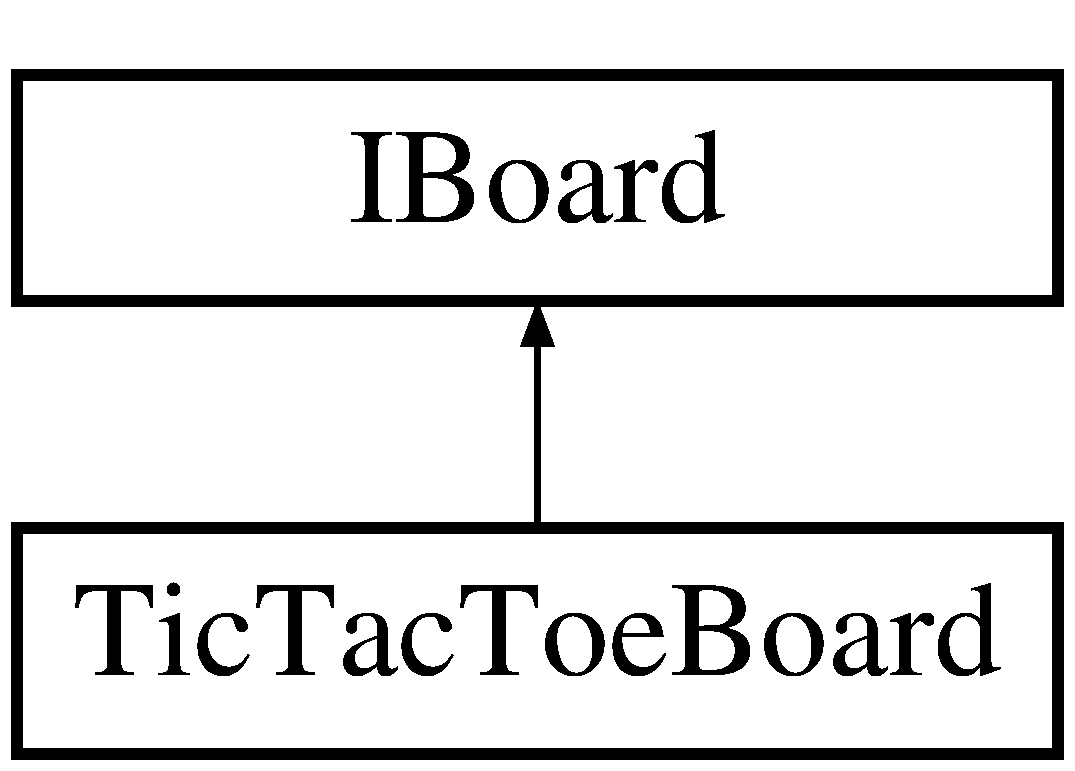
\includegraphics[height=2.000000cm]{class_tic_tac_toe_board}
\end{center}
\end{figure}
\subsection*{Public Member Functions}
\begin{DoxyCompactItemize}
\item 
\mbox{\Hypertarget{class_tic_tac_toe_board_adff1ee9118b05338cba02ba1f0352236}\label{class_tic_tac_toe_board_adff1ee9118b05338cba02ba1f0352236}} 
\hyperlink{class_tic_tac_toe_board_adff1ee9118b05338cba02ba1f0352236}{Tic\+Tac\+Toe\+Board} ()
\begin{DoxyCompactList}\small\item\em default constructor \end{DoxyCompactList}\item 
\mbox{\Hypertarget{class_tic_tac_toe_board_a6d5ab5e2d86f603927c3fa34d2fc03fc}\label{class_tic_tac_toe_board_a6d5ab5e2d86f603927c3fa34d2fc03fc}} 
\hyperlink{class_tic_tac_toe_board_a6d5ab5e2d86f603927c3fa34d2fc03fc}{$\sim$\+Tic\+Tac\+Toe\+Board} ()
\begin{DoxyCompactList}\small\item\em destructor \end{DoxyCompactList}\item 
\mbox{\Hypertarget{class_tic_tac_toe_board_a1800dd3903d95e8cd0eba839fbb06319}\label{class_tic_tac_toe_board_a1800dd3903d95e8cd0eba839fbb06319}} 
void \hyperlink{class_tic_tac_toe_board_a1800dd3903d95e8cd0eba839fbb06319}{init} ()
\begin{DoxyCompactList}\small\item\em init Initialize the board. \end{DoxyCompactList}\item 
\mbox{\Hypertarget{class_tic_tac_toe_board_ab4e17ab271aaf248e569297979b56f7a}\label{class_tic_tac_toe_board_ab4e17ab271aaf248e569297979b56f7a}} 
void \hyperlink{class_tic_tac_toe_board_ab4e17ab271aaf248e569297979b56f7a}{reset} ()
\begin{DoxyCompactList}\small\item\em reset Reset the board \end{DoxyCompactList}\item 
void \hyperlink{class_tic_tac_toe_board_a59fbbb4e8c7fa5ba6e1cdc8c33c50fb5}{play\+\_\+once} (int x, int y, int value)
\begin{DoxyCompactList}\small\item\em play\+\_\+once Select the given case and give the value to set it played by a player. \end{DoxyCompactList}\item 
\mbox{\Hypertarget{class_tic_tac_toe_board_aecc770d5451f2e3233da05859f6f37d4}\label{class_tic_tac_toe_board_aecc770d5451f2e3233da05859f6f37d4}} 
auto \hyperlink{class_tic_tac_toe_board_aecc770d5451f2e3233da05859f6f37d4}{get\+\_\+cases} () const
\begin{DoxyCompactList}\small\item\em get\+\_\+cases return access to the cases of the board. The Game\+Manager will need it to check winning conditions. \end{DoxyCompactList}\item 
bool \hyperlink{class_tic_tac_toe_board_a4d5be55d8439e66d32039ba98551fda7}{is\+\_\+full} () const
\begin{DoxyCompactList}\small\item\em is\+\_\+full Check if the board has used all its cases. \end{DoxyCompactList}\end{DoxyCompactItemize}


\subsection{Detailed Description}
\hyperlink{class_tic_tac_toe_board}{Tic\+Tac\+Toe\+Board} class will be holding the values for each each case of the board on a 3x3 for tictactoe. 

\subsection{Member Function Documentation}
\mbox{\Hypertarget{class_tic_tac_toe_board_a4d5be55d8439e66d32039ba98551fda7}\label{class_tic_tac_toe_board_a4d5be55d8439e66d32039ba98551fda7}} 
\index{Tic\+Tac\+Toe\+Board@{Tic\+Tac\+Toe\+Board}!is\+\_\+full@{is\+\_\+full}}
\index{is\+\_\+full@{is\+\_\+full}!Tic\+Tac\+Toe\+Board@{Tic\+Tac\+Toe\+Board}}
\subsubsection{\texorpdfstring{is\+\_\+full()}{is\_full()}}
{\footnotesize\ttfamily bool Tic\+Tac\+Toe\+Board\+::is\+\_\+full (\begin{DoxyParamCaption}{ }\end{DoxyParamCaption}) const\hspace{0.3cm}{\ttfamily [inline]}}



is\+\_\+full Check if the board has used all its cases. 

\begin{DoxyReturn}{Returns}
Return true if the board is fully used 
\end{DoxyReturn}
\mbox{\Hypertarget{class_tic_tac_toe_board_a59fbbb4e8c7fa5ba6e1cdc8c33c50fb5}\label{class_tic_tac_toe_board_a59fbbb4e8c7fa5ba6e1cdc8c33c50fb5}} 
\index{Tic\+Tac\+Toe\+Board@{Tic\+Tac\+Toe\+Board}!play\+\_\+once@{play\+\_\+once}}
\index{play\+\_\+once@{play\+\_\+once}!Tic\+Tac\+Toe\+Board@{Tic\+Tac\+Toe\+Board}}
\subsubsection{\texorpdfstring{play\+\_\+once()}{play\_once()}}
{\footnotesize\ttfamily void Tic\+Tac\+Toe\+Board\+::play\+\_\+once (\begin{DoxyParamCaption}\item[{int}]{x,  }\item[{int}]{y,  }\item[{int}]{value }\end{DoxyParamCaption})}



play\+\_\+once Select the given case and give the value to set it played by a player. 


\begin{DoxyParams}{Parameters}
{\em x} & X Coordinate to be played \\
\hline
{\em y} & Y Coordinate to be played \\
\hline
{\em value} & Value of the player (also called symbol). \\
\hline
\end{DoxyParams}


The documentation for this class was generated from the following files\+:\begin{DoxyCompactItemize}
\item 
Board/Tic\+Tac\+Toe\+Board.\+h\item 
Board/Tic\+Tac\+Toe\+Board.\+cpp\end{DoxyCompactItemize}

\hypertarget{class_tic_tac_toe_game_manager}{}\section{Tic\+Tac\+Toe\+Game\+Manager Class Reference}
\label{class_tic_tac_toe_game_manager}\index{Tic\+Tac\+Toe\+Game\+Manager@{Tic\+Tac\+Toe\+Game\+Manager}}


The \hyperlink{class_tic_tac_toe_game_manager}{Tic\+Tac\+Toe\+Game\+Manager} class This is the core of the application. This class is responsible of handling data creating, modification, winning condition etc.. It is the brain / core of the gameplay. Everything should pass through this singleton object.  




{\ttfamily \#include $<$Tic\+Tac\+Toe\+Game\+Manager.\+h$>$}

Inheritance diagram for Tic\+Tac\+Toe\+Game\+Manager\+:\begin{figure}[H]
\begin{center}
\leavevmode
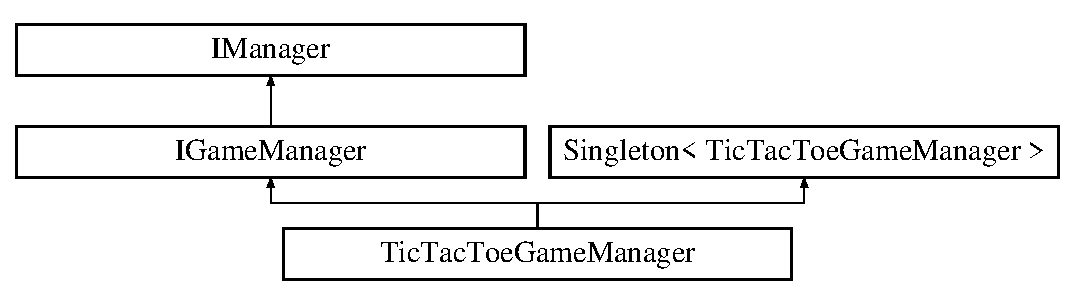
\includegraphics[height=3.000000cm]{class_tic_tac_toe_game_manager}
\end{center}
\end{figure}
\subsection*{Public Member Functions}
\begin{DoxyCompactItemize}
\item 
int \hyperlink{class_tic_tac_toe_game_manager_af276b6b66af26c170801bdd7aa1fd2f6}{play\+\_\+once} (int x, int y, class Q\+Push\+Button $\ast$button)
\begin{DoxyCompactList}\small\item\em play\+\_\+once Play once and check for different condition to make sure it is a possible move as well as checking if someone won the current round. \end{DoxyCompactList}\item 
bool \hyperlink{class_tic_tac_toe_game_manager_a4df4150f4292a51a8f711b3cf62e2608}{update\+\_\+score} (int winner\+Symbol)
\begin{DoxyCompactList}\small\item\em update\+\_\+score Update the score on both data (player score) as well as the ui. \end{DoxyCompactList}\item 
\mbox{\Hypertarget{class_tic_tac_toe_game_manager_a3dcf19f39ad3e65853c884bc29430460}\label{class_tic_tac_toe_game_manager_a3dcf19f39ad3e65853c884bc29430460}} 
void \hyperlink{class_tic_tac_toe_game_manager_a3dcf19f39ad3e65853c884bc29430460}{init} ()
\begin{DoxyCompactList}\small\item\em init Initialized the whole game. From player, board, score, data as well as UI. \end{DoxyCompactList}\item 
\mbox{\Hypertarget{class_tic_tac_toe_game_manager_a8d8d0b8f023beb5dab9357b263be44a9}\label{class_tic_tac_toe_game_manager_a8d8d0b8f023beb5dab9357b263be44a9}} 
void \hyperlink{class_tic_tac_toe_game_manager_a8d8d0b8f023beb5dab9357b263be44a9}{reset\+\_\+game} ()
\begin{DoxyCompactList}\small\item\em Reset the score and board to start a new round. \end{DoxyCompactList}\item 
void \hyperlink{class_tic_tac_toe_game_manager_a2d2b1cf7c29f760811f3ecc983dd2c5f}{create\+\_\+player} (const std\+::string \&name, const int \&symbol)
\begin{DoxyCompactList}\small\item\em create\+\_\+player Create a player based on its name and symbol. \end{DoxyCompactList}\item 
class \hyperlink{class_i_player}{I\+Player} $\ast$ \hyperlink{class_tic_tac_toe_game_manager_aacdb43d784567d95b535e66e91aca832}{get\+\_\+current\+\_\+player} ()
\begin{DoxyCompactList}\small\item\em get\+\_\+current\+\_\+player \end{DoxyCompactList}\item 
void \hyperlink{class_tic_tac_toe_game_manager_a309645c05a8ae25efc3d99729af9910b}{set\+\_\+max\+\_\+score} (const int \&max\+\_\+score)
\begin{DoxyCompactList}\small\item\em set\+\_\+max\+\_\+score Set the maximum score for th game. \end{DoxyCompactList}\item 
int \hyperlink{class_tic_tac_toe_game_manager_a311fdd7f83b66a5cc7eeafe584455315}{get\+\_\+max\+\_\+score} () const
\begin{DoxyCompactList}\small\item\em get\+\_\+max\+\_\+score \end{DoxyCompactList}\item 
class \hyperlink{class_i_player}{I\+Player} $\ast$ \hyperlink{class_tic_tac_toe_game_manager_a791389179603563f9c90a25aa173ceb4}{find\+\_\+player\+\_\+from\+\_\+symbol} (int symbol, int \&index)
\begin{DoxyCompactList}\small\item\em find\+\_\+player\+\_\+from\+\_\+symbol for the given symbol return the player and give its index as a reference parameter. \end{DoxyCompactList}\item 
std\+::vector$<$ class \hyperlink{class_i_player}{I\+Player} $\ast$ $>$ \hyperlink{class_tic_tac_toe_game_manager_ac7a54acc425dd27e92f8ff3866a333a6}{get\+\_\+players} () const
\begin{DoxyCompactList}\small\item\em get\+\_\+players \end{DoxyCompactList}\item 
\mbox{\Hypertarget{class_tic_tac_toe_game_manager_a2f3da6778543e6cf7b152570b7e1350d}\label{class_tic_tac_toe_game_manager_a2f3da6778543e6cf7b152570b7e1350d}} 
void {\bfseries set\+\_\+game\+\_\+window} (class \hyperlink{class_game_window}{Game\+Window} $\ast$gamewindow)
\end{DoxyCompactItemize}
\subsection*{Static Public Attributes}
\begin{DoxyCompactItemize}
\item 
\mbox{\Hypertarget{class_tic_tac_toe_game_manager_a23c11b057becb1c20a8e4f6c5389bf87}\label{class_tic_tac_toe_game_manager_a23c11b057becb1c20a8e4f6c5389bf87}} 
static const int \hyperlink{class_tic_tac_toe_game_manager_a23c11b057becb1c20a8e4f6c5389bf87}{s\+\_\+circle\+Pawn} = 1
\begin{DoxyCompactList}\small\item\em const variable used to define what is the circle value. \end{DoxyCompactList}\item 
\mbox{\Hypertarget{class_tic_tac_toe_game_manager_a34b41476fbb13bc8eec7b7f638524971}\label{class_tic_tac_toe_game_manager_a34b41476fbb13bc8eec7b7f638524971}} 
static const int \hyperlink{class_tic_tac_toe_game_manager_a34b41476fbb13bc8eec7b7f638524971}{s\+\_\+cross\+Pawn} = 2
\begin{DoxyCompactList}\small\item\em const variable used to define what is a cross value. \end{DoxyCompactList}\end{DoxyCompactItemize}
\subsection*{Protected Member Functions}
\begin{DoxyCompactItemize}
\item 
int \hyperlink{class_tic_tac_toe_game_manager_a25e9e556bf6f7324f4e7ef813778ecd0}{check\+\_\+vertical} ()
\begin{DoxyCompactList}\small\item\em check\+\_\+vertical \end{DoxyCompactList}\item 
int \hyperlink{class_tic_tac_toe_game_manager_af5045a121fc7c8f66bf8977ca2efb7b7}{check\+\_\+horizontal} ()
\begin{DoxyCompactList}\small\item\em check\+\_\+horizontal \end{DoxyCompactList}\item 
int \hyperlink{class_tic_tac_toe_game_manager_a7baa9e6ba971b930f8ace61cc42f034f}{check\+\_\+diagonal} ()
\begin{DoxyCompactList}\small\item\em check\+\_\+diagonal \end{DoxyCompactList}\item 
\mbox{\Hypertarget{class_tic_tac_toe_game_manager_a98277cf9aec99da101d1e81aece4ae5b}\label{class_tic_tac_toe_game_manager_a98277cf9aec99da101d1e81aece4ae5b}} 
void \hyperlink{class_tic_tac_toe_game_manager_a98277cf9aec99da101d1e81aece4ae5b}{get\+\_\+next\+\_\+player} ()
\begin{DoxyCompactList}\small\item\em get\+\_\+next\+\_\+player update the current player to be the next player. \end{DoxyCompactList}\item 
void \hyperlink{class_tic_tac_toe_game_manager_af97e0687582ed937fd01c603e82c2b5e}{set\+\_\+current\+\_\+player\+\_\+from\+\_\+index} (int index)
\begin{DoxyCompactList}\small\item\em set\+\_\+current\+\_\+player\+\_\+from\+\_\+index Set the current player to be for the given index. \end{DoxyCompactList}\item 
bool \hyperlink{class_tic_tac_toe_game_manager_aeac0a0f9d52ecf828f0827a2069e36ca}{check\+\_\+player\+\_\+score\+\_\+limit} ()
\begin{DoxyCompactList}\small\item\em check\+\_\+player\+\_\+score\+\_\+limit \end{DoxyCompactList}\item 
int \hyperlink{class_tic_tac_toe_game_manager_a6e619b1a463a7165949d34ce5d4ce1a7}{check\+\_\+winner} ()
\begin{DoxyCompactList}\small\item\em check\+\_\+winner \end{DoxyCompactList}\end{DoxyCompactItemize}
\subsection*{Friends}
\begin{DoxyCompactItemize}
\item 
\mbox{\Hypertarget{class_tic_tac_toe_game_manager_ad810229015d6649556c3e37f689094f0}\label{class_tic_tac_toe_game_manager_ad810229015d6649556c3e37f689094f0}} 
class {\bfseries Singleton$<$ Tic\+Tac\+Toe\+Game\+Manager $>$}
\end{DoxyCompactItemize}
\subsection*{Additional Inherited Members}


\subsection{Detailed Description}
The \hyperlink{class_tic_tac_toe_game_manager}{Tic\+Tac\+Toe\+Game\+Manager} class This is the core of the application. This class is responsible of handling data creating, modification, winning condition etc.. It is the brain / core of the gameplay. Everything should pass through this singleton object. 

\subsection{Member Function Documentation}
\mbox{\Hypertarget{class_tic_tac_toe_game_manager_a7baa9e6ba971b930f8ace61cc42f034f}\label{class_tic_tac_toe_game_manager_a7baa9e6ba971b930f8ace61cc42f034f}} 
\index{Tic\+Tac\+Toe\+Game\+Manager@{Tic\+Tac\+Toe\+Game\+Manager}!check\+\_\+diagonal@{check\+\_\+diagonal}}
\index{check\+\_\+diagonal@{check\+\_\+diagonal}!Tic\+Tac\+Toe\+Game\+Manager@{Tic\+Tac\+Toe\+Game\+Manager}}
\subsubsection{\texorpdfstring{check\+\_\+diagonal()}{check\_diagonal()}}
{\footnotesize\ttfamily int Tic\+Tac\+Toe\+Game\+Manager\+::check\+\_\+diagonal (\begin{DoxyParamCaption}{ }\end{DoxyParamCaption})\hspace{0.3cm}{\ttfamily [protected]}}



check\+\_\+diagonal 

\begin{DoxyReturn}{Returns}
return more than 0 if a player won on the diagonal. 
\end{DoxyReturn}
\mbox{\Hypertarget{class_tic_tac_toe_game_manager_af5045a121fc7c8f66bf8977ca2efb7b7}\label{class_tic_tac_toe_game_manager_af5045a121fc7c8f66bf8977ca2efb7b7}} 
\index{Tic\+Tac\+Toe\+Game\+Manager@{Tic\+Tac\+Toe\+Game\+Manager}!check\+\_\+horizontal@{check\+\_\+horizontal}}
\index{check\+\_\+horizontal@{check\+\_\+horizontal}!Tic\+Tac\+Toe\+Game\+Manager@{Tic\+Tac\+Toe\+Game\+Manager}}
\subsubsection{\texorpdfstring{check\+\_\+horizontal()}{check\_horizontal()}}
{\footnotesize\ttfamily int Tic\+Tac\+Toe\+Game\+Manager\+::check\+\_\+horizontal (\begin{DoxyParamCaption}{ }\end{DoxyParamCaption})\hspace{0.3cm}{\ttfamily [protected]}}



check\+\_\+horizontal 

\begin{DoxyReturn}{Returns}
return more than 0 if a player won horizontaly. 
\end{DoxyReturn}
\mbox{\Hypertarget{class_tic_tac_toe_game_manager_aeac0a0f9d52ecf828f0827a2069e36ca}\label{class_tic_tac_toe_game_manager_aeac0a0f9d52ecf828f0827a2069e36ca}} 
\index{Tic\+Tac\+Toe\+Game\+Manager@{Tic\+Tac\+Toe\+Game\+Manager}!check\+\_\+player\+\_\+score\+\_\+limit@{check\+\_\+player\+\_\+score\+\_\+limit}}
\index{check\+\_\+player\+\_\+score\+\_\+limit@{check\+\_\+player\+\_\+score\+\_\+limit}!Tic\+Tac\+Toe\+Game\+Manager@{Tic\+Tac\+Toe\+Game\+Manager}}
\subsubsection{\texorpdfstring{check\+\_\+player\+\_\+score\+\_\+limit()}{check\_player\_score\_limit()}}
{\footnotesize\ttfamily bool Tic\+Tac\+Toe\+Game\+Manager\+::check\+\_\+player\+\_\+score\+\_\+limit (\begin{DoxyParamCaption}{ }\end{DoxyParamCaption})\hspace{0.3cm}{\ttfamily [protected]}}



check\+\_\+player\+\_\+score\+\_\+limit 

\begin{DoxyReturn}{Returns}
return true if one of the player reached the score limit. This should end the game. 
\end{DoxyReturn}
\mbox{\Hypertarget{class_tic_tac_toe_game_manager_a25e9e556bf6f7324f4e7ef813778ecd0}\label{class_tic_tac_toe_game_manager_a25e9e556bf6f7324f4e7ef813778ecd0}} 
\index{Tic\+Tac\+Toe\+Game\+Manager@{Tic\+Tac\+Toe\+Game\+Manager}!check\+\_\+vertical@{check\+\_\+vertical}}
\index{check\+\_\+vertical@{check\+\_\+vertical}!Tic\+Tac\+Toe\+Game\+Manager@{Tic\+Tac\+Toe\+Game\+Manager}}
\subsubsection{\texorpdfstring{check\+\_\+vertical()}{check\_vertical()}}
{\footnotesize\ttfamily int Tic\+Tac\+Toe\+Game\+Manager\+::check\+\_\+vertical (\begin{DoxyParamCaption}{ }\end{DoxyParamCaption})\hspace{0.3cm}{\ttfamily [protected]}}



check\+\_\+vertical 

\begin{DoxyReturn}{Returns}
return more than 0 if a player won verticaly. 
\end{DoxyReturn}
\mbox{\Hypertarget{class_tic_tac_toe_game_manager_a6e619b1a463a7165949d34ce5d4ce1a7}\label{class_tic_tac_toe_game_manager_a6e619b1a463a7165949d34ce5d4ce1a7}} 
\index{Tic\+Tac\+Toe\+Game\+Manager@{Tic\+Tac\+Toe\+Game\+Manager}!check\+\_\+winner@{check\+\_\+winner}}
\index{check\+\_\+winner@{check\+\_\+winner}!Tic\+Tac\+Toe\+Game\+Manager@{Tic\+Tac\+Toe\+Game\+Manager}}
\subsubsection{\texorpdfstring{check\+\_\+winner()}{check\_winner()}}
{\footnotesize\ttfamily int Tic\+Tac\+Toe\+Game\+Manager\+::check\+\_\+winner (\begin{DoxyParamCaption}{ }\end{DoxyParamCaption})\hspace{0.3cm}{\ttfamily [protected]}}



check\+\_\+winner 

\begin{DoxyReturn}{Returns}
Return more than 0 if a player won the current round. 
\end{DoxyReturn}
\mbox{\Hypertarget{class_tic_tac_toe_game_manager_a2d2b1cf7c29f760811f3ecc983dd2c5f}\label{class_tic_tac_toe_game_manager_a2d2b1cf7c29f760811f3ecc983dd2c5f}} 
\index{Tic\+Tac\+Toe\+Game\+Manager@{Tic\+Tac\+Toe\+Game\+Manager}!create\+\_\+player@{create\+\_\+player}}
\index{create\+\_\+player@{create\+\_\+player}!Tic\+Tac\+Toe\+Game\+Manager@{Tic\+Tac\+Toe\+Game\+Manager}}
\subsubsection{\texorpdfstring{create\+\_\+player()}{create\_player()}}
{\footnotesize\ttfamily void Tic\+Tac\+Toe\+Game\+Manager\+::create\+\_\+player (\begin{DoxyParamCaption}\item[{const std\+::string \&}]{name,  }\item[{const int \&}]{symbol }\end{DoxyParamCaption})\hspace{0.3cm}{\ttfamily [virtual]}}



create\+\_\+player Create a player based on its name and symbol. 


\begin{DoxyParams}{Parameters}
{\em name} & Name of the player \\
\hline
{\em symbol} & Symbol (either cross or Circle) of the player. \\
\hline
\end{DoxyParams}


Implements \hyperlink{class_i_game_manager_a197ed85a1deadeb414b3030e11d0bf1e}{I\+Game\+Manager}.

\mbox{\Hypertarget{class_tic_tac_toe_game_manager_a791389179603563f9c90a25aa173ceb4}\label{class_tic_tac_toe_game_manager_a791389179603563f9c90a25aa173ceb4}} 
\index{Tic\+Tac\+Toe\+Game\+Manager@{Tic\+Tac\+Toe\+Game\+Manager}!find\+\_\+player\+\_\+from\+\_\+symbol@{find\+\_\+player\+\_\+from\+\_\+symbol}}
\index{find\+\_\+player\+\_\+from\+\_\+symbol@{find\+\_\+player\+\_\+from\+\_\+symbol}!Tic\+Tac\+Toe\+Game\+Manager@{Tic\+Tac\+Toe\+Game\+Manager}}
\subsubsection{\texorpdfstring{find\+\_\+player\+\_\+from\+\_\+symbol()}{find\_player\_from\_symbol()}}
{\footnotesize\ttfamily \hyperlink{class_i_player}{I\+Player} $\ast$ Tic\+Tac\+Toe\+Game\+Manager\+::find\+\_\+player\+\_\+from\+\_\+symbol (\begin{DoxyParamCaption}\item[{int}]{symbol,  }\item[{int \&}]{index }\end{DoxyParamCaption})}



find\+\_\+player\+\_\+from\+\_\+symbol for the given symbol return the player and give its index as a reference parameter. 


\begin{DoxyParams}{Parameters}
{\em symbol} & symbol of the player \\
\hline
{\em index} & reference to the index of the player (in parameter). \\
\hline
\end{DoxyParams}
\begin{DoxyReturn}{Returns}

\end{DoxyReturn}
\mbox{\Hypertarget{class_tic_tac_toe_game_manager_aacdb43d784567d95b535e66e91aca832}\label{class_tic_tac_toe_game_manager_aacdb43d784567d95b535e66e91aca832}} 
\index{Tic\+Tac\+Toe\+Game\+Manager@{Tic\+Tac\+Toe\+Game\+Manager}!get\+\_\+current\+\_\+player@{get\+\_\+current\+\_\+player}}
\index{get\+\_\+current\+\_\+player@{get\+\_\+current\+\_\+player}!Tic\+Tac\+Toe\+Game\+Manager@{Tic\+Tac\+Toe\+Game\+Manager}}
\subsubsection{\texorpdfstring{get\+\_\+current\+\_\+player()}{get\_current\_player()}}
{\footnotesize\ttfamily class \hyperlink{class_i_player}{I\+Player}$\ast$ Tic\+Tac\+Toe\+Game\+Manager\+::get\+\_\+current\+\_\+player (\begin{DoxyParamCaption}{ }\end{DoxyParamCaption})\hspace{0.3cm}{\ttfamily [inline]}}



get\+\_\+current\+\_\+player 

\begin{DoxyReturn}{Returns}
Return the currenty player. 
\end{DoxyReturn}
\mbox{\Hypertarget{class_tic_tac_toe_game_manager_a311fdd7f83b66a5cc7eeafe584455315}\label{class_tic_tac_toe_game_manager_a311fdd7f83b66a5cc7eeafe584455315}} 
\index{Tic\+Tac\+Toe\+Game\+Manager@{Tic\+Tac\+Toe\+Game\+Manager}!get\+\_\+max\+\_\+score@{get\+\_\+max\+\_\+score}}
\index{get\+\_\+max\+\_\+score@{get\+\_\+max\+\_\+score}!Tic\+Tac\+Toe\+Game\+Manager@{Tic\+Tac\+Toe\+Game\+Manager}}
\subsubsection{\texorpdfstring{get\+\_\+max\+\_\+score()}{get\_max\_score()}}
{\footnotesize\ttfamily int Tic\+Tac\+Toe\+Game\+Manager\+::get\+\_\+max\+\_\+score (\begin{DoxyParamCaption}{ }\end{DoxyParamCaption}) const\hspace{0.3cm}{\ttfamily [inline]}}



get\+\_\+max\+\_\+score 

\begin{DoxyReturn}{Returns}
return the max score. 
\end{DoxyReturn}
\mbox{\Hypertarget{class_tic_tac_toe_game_manager_ac7a54acc425dd27e92f8ff3866a333a6}\label{class_tic_tac_toe_game_manager_ac7a54acc425dd27e92f8ff3866a333a6}} 
\index{Tic\+Tac\+Toe\+Game\+Manager@{Tic\+Tac\+Toe\+Game\+Manager}!get\+\_\+players@{get\+\_\+players}}
\index{get\+\_\+players@{get\+\_\+players}!Tic\+Tac\+Toe\+Game\+Manager@{Tic\+Tac\+Toe\+Game\+Manager}}
\subsubsection{\texorpdfstring{get\+\_\+players()}{get\_players()}}
{\footnotesize\ttfamily std\+::vector$<$class \hyperlink{class_i_player}{I\+Player}$\ast$$>$ Tic\+Tac\+Toe\+Game\+Manager\+::get\+\_\+players (\begin{DoxyParamCaption}{ }\end{DoxyParamCaption}) const\hspace{0.3cm}{\ttfamily [inline]}}



get\+\_\+players 

\begin{DoxyReturn}{Returns}
return the players of the game. 
\end{DoxyReturn}
\mbox{\Hypertarget{class_tic_tac_toe_game_manager_af276b6b66af26c170801bdd7aa1fd2f6}\label{class_tic_tac_toe_game_manager_af276b6b66af26c170801bdd7aa1fd2f6}} 
\index{Tic\+Tac\+Toe\+Game\+Manager@{Tic\+Tac\+Toe\+Game\+Manager}!play\+\_\+once@{play\+\_\+once}}
\index{play\+\_\+once@{play\+\_\+once}!Tic\+Tac\+Toe\+Game\+Manager@{Tic\+Tac\+Toe\+Game\+Manager}}
\subsubsection{\texorpdfstring{play\+\_\+once()}{play\_once()}}
{\footnotesize\ttfamily int Tic\+Tac\+Toe\+Game\+Manager\+::play\+\_\+once (\begin{DoxyParamCaption}\item[{int}]{x,  }\item[{int}]{y,  }\item[{class Q\+Push\+Button $\ast$}]{button }\end{DoxyParamCaption})}



play\+\_\+once Play once and check for different condition to make sure it is a possible move as well as checking if someone won the current round. 


\begin{DoxyParams}{Parameters}
{\em x} & Position on the X axis. \\
\hline
{\em y} & Position on the Y axis \\
\hline
{\em button} & Pointer to the current button in the UI that has been selected so we can update the UI. \\
\hline
\end{DoxyParams}
\begin{DoxyReturn}{Returns}
return -\/1 if something went wrong other return the symbol of the player. 
\end{DoxyReturn}
\mbox{\Hypertarget{class_tic_tac_toe_game_manager_af97e0687582ed937fd01c603e82c2b5e}\label{class_tic_tac_toe_game_manager_af97e0687582ed937fd01c603e82c2b5e}} 
\index{Tic\+Tac\+Toe\+Game\+Manager@{Tic\+Tac\+Toe\+Game\+Manager}!set\+\_\+current\+\_\+player\+\_\+from\+\_\+index@{set\+\_\+current\+\_\+player\+\_\+from\+\_\+index}}
\index{set\+\_\+current\+\_\+player\+\_\+from\+\_\+index@{set\+\_\+current\+\_\+player\+\_\+from\+\_\+index}!Tic\+Tac\+Toe\+Game\+Manager@{Tic\+Tac\+Toe\+Game\+Manager}}
\subsubsection{\texorpdfstring{set\+\_\+current\+\_\+player\+\_\+from\+\_\+index()}{set\_current\_player\_from\_index()}}
{\footnotesize\ttfamily void Tic\+Tac\+Toe\+Game\+Manager\+::set\+\_\+current\+\_\+player\+\_\+from\+\_\+index (\begin{DoxyParamCaption}\item[{int}]{index }\end{DoxyParamCaption})\hspace{0.3cm}{\ttfamily [protected]}}



set\+\_\+current\+\_\+player\+\_\+from\+\_\+index Set the current player to be for the given index. 


\begin{DoxyParams}{Parameters}
{\em index} & index of the current player to be set. \\
\hline
\end{DoxyParams}
\mbox{\Hypertarget{class_tic_tac_toe_game_manager_a309645c05a8ae25efc3d99729af9910b}\label{class_tic_tac_toe_game_manager_a309645c05a8ae25efc3d99729af9910b}} 
\index{Tic\+Tac\+Toe\+Game\+Manager@{Tic\+Tac\+Toe\+Game\+Manager}!set\+\_\+max\+\_\+score@{set\+\_\+max\+\_\+score}}
\index{set\+\_\+max\+\_\+score@{set\+\_\+max\+\_\+score}!Tic\+Tac\+Toe\+Game\+Manager@{Tic\+Tac\+Toe\+Game\+Manager}}
\subsubsection{\texorpdfstring{set\+\_\+max\+\_\+score()}{set\_max\_score()}}
{\footnotesize\ttfamily void Tic\+Tac\+Toe\+Game\+Manager\+::set\+\_\+max\+\_\+score (\begin{DoxyParamCaption}\item[{const int \&}]{max\+\_\+score }\end{DoxyParamCaption})\hspace{0.3cm}{\ttfamily [inline]}}



set\+\_\+max\+\_\+score Set the maximum score for th game. 


\begin{DoxyParams}{Parameters}
{\em max\+\_\+score} & Maximum integer to be used. Depending on the widget limit \\
\hline
\end{DoxyParams}
\mbox{\Hypertarget{class_tic_tac_toe_game_manager_a4df4150f4292a51a8f711b3cf62e2608}\label{class_tic_tac_toe_game_manager_a4df4150f4292a51a8f711b3cf62e2608}} 
\index{Tic\+Tac\+Toe\+Game\+Manager@{Tic\+Tac\+Toe\+Game\+Manager}!update\+\_\+score@{update\+\_\+score}}
\index{update\+\_\+score@{update\+\_\+score}!Tic\+Tac\+Toe\+Game\+Manager@{Tic\+Tac\+Toe\+Game\+Manager}}
\subsubsection{\texorpdfstring{update\+\_\+score()}{update\_score()}}
{\footnotesize\ttfamily bool Tic\+Tac\+Toe\+Game\+Manager\+::update\+\_\+score (\begin{DoxyParamCaption}\item[{int}]{winner\+Symbol }\end{DoxyParamCaption})}



update\+\_\+score Update the score on both data (player score) as well as the ui. 


\begin{DoxyParams}{Parameters}
{\em winner\+Symbol} & Takes the current symbol of the winner (last played symbol). \\
\hline
\end{DoxyParams}
\begin{DoxyReturn}{Returns}
return true if it was updated. 
\end{DoxyReturn}


The documentation for this class was generated from the following files\+:\begin{DoxyCompactItemize}
\item 
Manager/Tic\+Tac\+Toe\+Game\+Manager.\+h\item 
Manager/Tic\+Tac\+Toe\+Game\+Manager.\+cpp\end{DoxyCompactItemize}

\hypertarget{class_tic_tac_toe_player}{}\section{Tic\+Tac\+Toe\+Player Class Reference}
\label{class_tic_tac_toe_player}\index{Tic\+Tac\+Toe\+Player@{Tic\+Tac\+Toe\+Player}}


The \hyperlink{class_tic_tac_toe_player}{Tic\+Tac\+Toe\+Player} class.  




{\ttfamily \#include $<$Tic\+Tac\+Toe\+Player.\+h$>$}

Inheritance diagram for Tic\+Tac\+Toe\+Player\+:\begin{figure}[H]
\begin{center}
\leavevmode
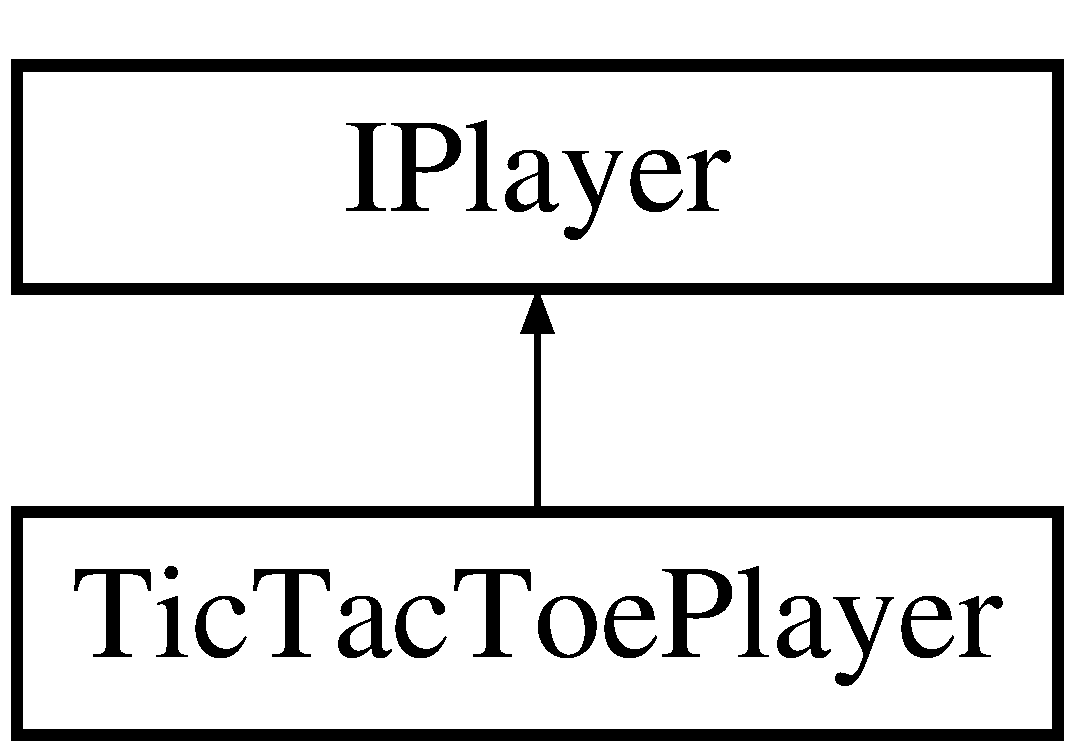
\includegraphics[height=2.000000cm]{class_tic_tac_toe_player}
\end{center}
\end{figure}
\subsection*{Public Member Functions}
\begin{DoxyCompactItemize}
\item 
\mbox{\Hypertarget{class_tic_tac_toe_player_a72a0abd8463de646675b1b7f585c9170}\label{class_tic_tac_toe_player_a72a0abd8463de646675b1b7f585c9170}} 
\hyperlink{class_tic_tac_toe_player_a72a0abd8463de646675b1b7f585c9170}{Tic\+Tac\+Toe\+Player} ()
\begin{DoxyCompactList}\small\item\em \hyperlink{class_tic_tac_toe_player}{Tic\+Tac\+Toe\+Player} Default constructor. \end{DoxyCompactList}\item 
\hyperlink{class_tic_tac_toe_player_a6ed50322b8f71dfb0f6ce067d33ff376}{Tic\+Tac\+Toe\+Player} (const std\+::string \&name, int symbol)
\begin{DoxyCompactList}\small\item\em \hyperlink{class_tic_tac_toe_player}{Tic\+Tac\+Toe\+Player} Parametrized constructor. \end{DoxyCompactList}\item 
\mbox{\Hypertarget{class_tic_tac_toe_player_a3ba5ea5d34cd49ca04b3929e9785d394}\label{class_tic_tac_toe_player_a3ba5ea5d34cd49ca04b3929e9785d394}} 
\hyperlink{class_tic_tac_toe_player_a3ba5ea5d34cd49ca04b3929e9785d394}{$\sim$\+Tic\+Tac\+Toe\+Player} ()
\begin{DoxyCompactList}\small\item\em Destructor. \end{DoxyCompactList}\item 
void \hyperlink{class_tic_tac_toe_player_a0f2c55f9e76fa53cf723735253dfc43e}{set\+\_\+name} (const std\+::string \&name)
\begin{DoxyCompactList}\small\item\em set\+\_\+name Set the name of the player \end{DoxyCompactList}\item 
std\+::string \hyperlink{class_tic_tac_toe_player_ace0eccd41811e4345ed6bccdb623e6e7}{get\+\_\+name} () const
\begin{DoxyCompactList}\small\item\em get\+\_\+name Get the name of the player \end{DoxyCompactList}\item 
int \hyperlink{class_tic_tac_toe_player_ad0f195090b263ae0ec24019edfeb9f3d}{get\+\_\+score} () const
\begin{DoxyCompactList}\small\item\em get\+\_\+score Get the score of the player \end{DoxyCompactList}\item 
int \hyperlink{class_tic_tac_toe_player_a5e73a7154c82e2a09f1b89e5e5d70796}{get\+\_\+symbol} () const
\begin{DoxyCompactList}\small\item\em get\+\_\+symbol Get the symbol of the player \end{DoxyCompactList}\item 
\mbox{\Hypertarget{class_tic_tac_toe_player_a98589a86842d7c49b082fd3449bd3ba3}\label{class_tic_tac_toe_player_a98589a86842d7c49b082fd3449bd3ba3}} 
void \hyperlink{class_tic_tac_toe_player_a98589a86842d7c49b082fd3449bd3ba3}{update\+\_\+score} ()
\begin{DoxyCompactList}\small\item\em update\+\_\+score Update the score of the player \end{DoxyCompactList}\item 
\mbox{\Hypertarget{class_tic_tac_toe_player_a7fbb25d79fc17351288bcf0298605f3b}\label{class_tic_tac_toe_player_a7fbb25d79fc17351288bcf0298605f3b}} 
void \hyperlink{class_tic_tac_toe_player_a7fbb25d79fc17351288bcf0298605f3b}{reset\+\_\+score} ()
\begin{DoxyCompactList}\small\item\em reset\+\_\+score Reset the score of the player. \end{DoxyCompactList}\end{DoxyCompactItemize}
\subsection*{Protected Attributes}
\begin{DoxyCompactItemize}
\item 
\mbox{\Hypertarget{class_tic_tac_toe_player_ad2f56b8e5337362b6b0effc05fd7633e}\label{class_tic_tac_toe_player_ad2f56b8e5337362b6b0effc05fd7633e}} 
std\+::string \hyperlink{class_tic_tac_toe_player_ad2f56b8e5337362b6b0effc05fd7633e}{m\+\_\+name}
\begin{DoxyCompactList}\small\item\em name of the player \end{DoxyCompactList}\item 
\mbox{\Hypertarget{class_tic_tac_toe_player_a931f1c29bf11a6dd32552ed8b8afcccc}\label{class_tic_tac_toe_player_a931f1c29bf11a6dd32552ed8b8afcccc}} 
\hyperlink{class_tic_tac_toe_score}{Tic\+Tac\+Toe\+Score} \hyperlink{class_tic_tac_toe_player_a931f1c29bf11a6dd32552ed8b8afcccc}{m\+\_\+score}
\begin{DoxyCompactList}\small\item\em score of the player \end{DoxyCompactList}\item 
\mbox{\Hypertarget{class_tic_tac_toe_player_abe8d693d11fc49191a8f664485875693}\label{class_tic_tac_toe_player_abe8d693d11fc49191a8f664485875693}} 
int \hyperlink{class_tic_tac_toe_player_abe8d693d11fc49191a8f664485875693}{m\+\_\+symbol}
\begin{DoxyCompactList}\small\item\em symbol of the player \end{DoxyCompactList}\end{DoxyCompactItemize}


\subsection{Detailed Description}
The \hyperlink{class_tic_tac_toe_player}{Tic\+Tac\+Toe\+Player} class. 

\subsection{Constructor \& Destructor Documentation}
\mbox{\Hypertarget{class_tic_tac_toe_player_a6ed50322b8f71dfb0f6ce067d33ff376}\label{class_tic_tac_toe_player_a6ed50322b8f71dfb0f6ce067d33ff376}} 
\index{Tic\+Tac\+Toe\+Player@{Tic\+Tac\+Toe\+Player}!Tic\+Tac\+Toe\+Player@{Tic\+Tac\+Toe\+Player}}
\index{Tic\+Tac\+Toe\+Player@{Tic\+Tac\+Toe\+Player}!Tic\+Tac\+Toe\+Player@{Tic\+Tac\+Toe\+Player}}
\subsubsection{\texorpdfstring{Tic\+Tac\+Toe\+Player()}{TicTacToePlayer()}}
{\footnotesize\ttfamily Tic\+Tac\+Toe\+Player\+::\+Tic\+Tac\+Toe\+Player (\begin{DoxyParamCaption}\item[{const std\+::string \&}]{name,  }\item[{int}]{symbol }\end{DoxyParamCaption})\hspace{0.3cm}{\ttfamily [inline]}}



\hyperlink{class_tic_tac_toe_player}{Tic\+Tac\+Toe\+Player} Parametrized constructor. 


\begin{DoxyParams}{Parameters}
{\em name} & Name of the player \\
\hline
{\em symbol} & Symbol of the player \\
\hline
\end{DoxyParams}


\subsection{Member Function Documentation}
\mbox{\Hypertarget{class_tic_tac_toe_player_ace0eccd41811e4345ed6bccdb623e6e7}\label{class_tic_tac_toe_player_ace0eccd41811e4345ed6bccdb623e6e7}} 
\index{Tic\+Tac\+Toe\+Player@{Tic\+Tac\+Toe\+Player}!get\+\_\+name@{get\+\_\+name}}
\index{get\+\_\+name@{get\+\_\+name}!Tic\+Tac\+Toe\+Player@{Tic\+Tac\+Toe\+Player}}
\subsubsection{\texorpdfstring{get\+\_\+name()}{get\_name()}}
{\footnotesize\ttfamily std\+::string Tic\+Tac\+Toe\+Player\+::get\+\_\+name (\begin{DoxyParamCaption}{ }\end{DoxyParamCaption}) const\hspace{0.3cm}{\ttfamily [inline]}, {\ttfamily [virtual]}}



get\+\_\+name Get the name of the player 

\begin{DoxyReturn}{Returns}
the name of the player. 
\end{DoxyReturn}


Implements \hyperlink{class_i_player}{I\+Player}.

\mbox{\Hypertarget{class_tic_tac_toe_player_ad0f195090b263ae0ec24019edfeb9f3d}\label{class_tic_tac_toe_player_ad0f195090b263ae0ec24019edfeb9f3d}} 
\index{Tic\+Tac\+Toe\+Player@{Tic\+Tac\+Toe\+Player}!get\+\_\+score@{get\+\_\+score}}
\index{get\+\_\+score@{get\+\_\+score}!Tic\+Tac\+Toe\+Player@{Tic\+Tac\+Toe\+Player}}
\subsubsection{\texorpdfstring{get\+\_\+score()}{get\_score()}}
{\footnotesize\ttfamily int Tic\+Tac\+Toe\+Player\+::get\+\_\+score (\begin{DoxyParamCaption}{ }\end{DoxyParamCaption}) const\hspace{0.3cm}{\ttfamily [inline]}, {\ttfamily [virtual]}}



get\+\_\+score Get the score of the player 

\begin{DoxyReturn}{Returns}
return the score of the player 
\end{DoxyReturn}


Implements \hyperlink{class_i_player}{I\+Player}.

\mbox{\Hypertarget{class_tic_tac_toe_player_a5e73a7154c82e2a09f1b89e5e5d70796}\label{class_tic_tac_toe_player_a5e73a7154c82e2a09f1b89e5e5d70796}} 
\index{Tic\+Tac\+Toe\+Player@{Tic\+Tac\+Toe\+Player}!get\+\_\+symbol@{get\+\_\+symbol}}
\index{get\+\_\+symbol@{get\+\_\+symbol}!Tic\+Tac\+Toe\+Player@{Tic\+Tac\+Toe\+Player}}
\subsubsection{\texorpdfstring{get\+\_\+symbol()}{get\_symbol()}}
{\footnotesize\ttfamily int Tic\+Tac\+Toe\+Player\+::get\+\_\+symbol (\begin{DoxyParamCaption}{ }\end{DoxyParamCaption}) const\hspace{0.3cm}{\ttfamily [inline]}, {\ttfamily [virtual]}}



get\+\_\+symbol Get the symbol of the player 

\begin{DoxyReturn}{Returns}
return the symbol of the player 
\end{DoxyReturn}


Implements \hyperlink{class_i_player}{I\+Player}.

\mbox{\Hypertarget{class_tic_tac_toe_player_a0f2c55f9e76fa53cf723735253dfc43e}\label{class_tic_tac_toe_player_a0f2c55f9e76fa53cf723735253dfc43e}} 
\index{Tic\+Tac\+Toe\+Player@{Tic\+Tac\+Toe\+Player}!set\+\_\+name@{set\+\_\+name}}
\index{set\+\_\+name@{set\+\_\+name}!Tic\+Tac\+Toe\+Player@{Tic\+Tac\+Toe\+Player}}
\subsubsection{\texorpdfstring{set\+\_\+name()}{set\_name()}}
{\footnotesize\ttfamily void Tic\+Tac\+Toe\+Player\+::set\+\_\+name (\begin{DoxyParamCaption}\item[{const std\+::string \&}]{name }\end{DoxyParamCaption})\hspace{0.3cm}{\ttfamily [inline]}, {\ttfamily [virtual]}}



set\+\_\+name Set the name of the player 


\begin{DoxyParams}{Parameters}
{\em name} & of the player \\
\hline
\end{DoxyParams}


Implements \hyperlink{class_i_player}{I\+Player}.



The documentation for this class was generated from the following file\+:\begin{DoxyCompactItemize}
\item 
Player/Tic\+Tac\+Toe\+Player.\+h\end{DoxyCompactItemize}

\hypertarget{class_tic_tac_toe_score}{}\section{Tic\+Tac\+Toe\+Score Class Reference}
\label{class_tic_tac_toe_score}\index{Tic\+Tac\+Toe\+Score@{Tic\+Tac\+Toe\+Score}}


The \hyperlink{class_tic_tac_toe_score}{Tic\+Tac\+Toe\+Score} class Implement the way a score is calculate for a Tic\+Tac\+Toe game. More information about this design can be found looking at the Strategy Pattern.  




{\ttfamily \#include $<$Tic\+Tac\+Toe\+Score.\+h$>$}

Inheritance diagram for Tic\+Tac\+Toe\+Score\+:\begin{figure}[H]
\begin{center}
\leavevmode
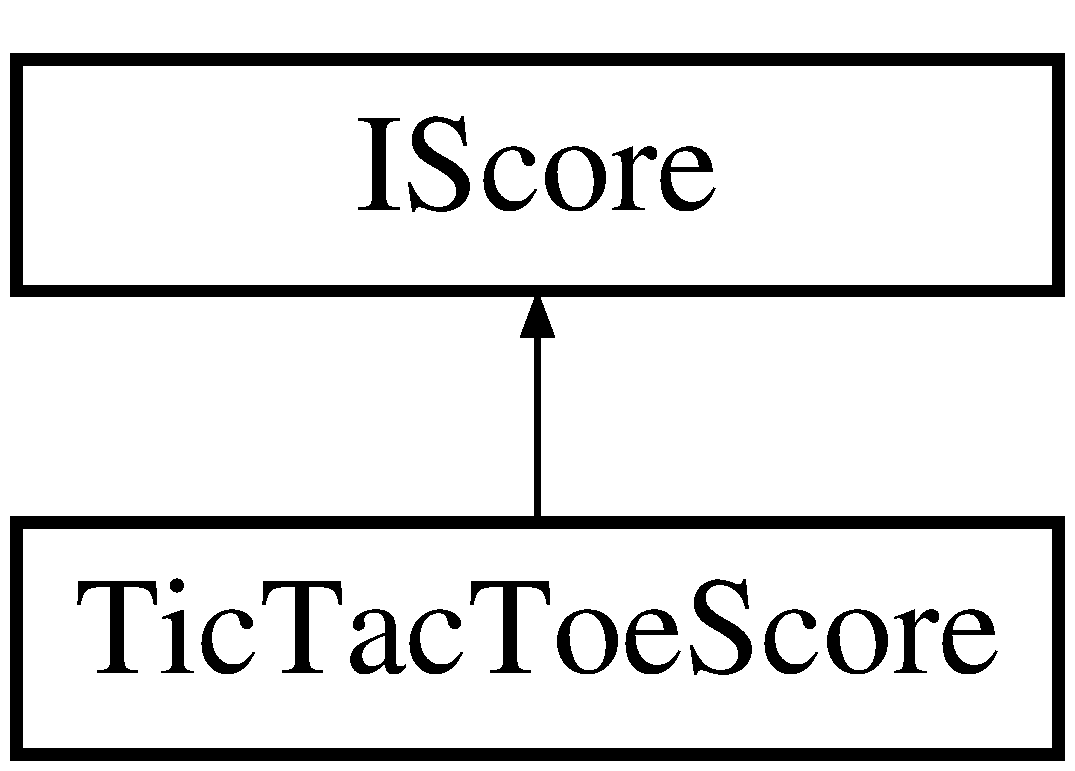
\includegraphics[height=2.000000cm]{class_tic_tac_toe_score}
\end{center}
\end{figure}
\subsection*{Public Member Functions}
\begin{DoxyCompactItemize}
\item 
\mbox{\Hypertarget{class_tic_tac_toe_score_a722bc40d54bbfd0e7835b478d8f0a38d}\label{class_tic_tac_toe_score_a722bc40d54bbfd0e7835b478d8f0a38d}} 
\hyperlink{class_tic_tac_toe_score_a722bc40d54bbfd0e7835b478d8f0a38d}{Tic\+Tac\+Toe\+Score} ()
\begin{DoxyCompactList}\small\item\em Constructor. \end{DoxyCompactList}\item 
\mbox{\Hypertarget{class_tic_tac_toe_score_aa5efe0e9673d7e8d89dc51c4174f87ee}\label{class_tic_tac_toe_score_aa5efe0e9673d7e8d89dc51c4174f87ee}} 
\hyperlink{class_tic_tac_toe_score_aa5efe0e9673d7e8d89dc51c4174f87ee}{$\sim$\+Tic\+Tac\+Toe\+Score} ()
\begin{DoxyCompactList}\small\item\em Destructor. \end{DoxyCompactList}\item 
\mbox{\Hypertarget{class_tic_tac_toe_score_a463b691c79c6f566f98ab415cfa6bad4}\label{class_tic_tac_toe_score_a463b691c79c6f566f98ab415cfa6bad4}} 
void \hyperlink{class_tic_tac_toe_score_a463b691c79c6f566f98ab415cfa6bad4}{init} ()
\begin{DoxyCompactList}\small\item\em init Initialize the score. \end{DoxyCompactList}\item 
\mbox{\Hypertarget{class_tic_tac_toe_score_a4475a34d15caf4b0bd31297583f5395a}\label{class_tic_tac_toe_score_a4475a34d15caf4b0bd31297583f5395a}} 
void \hyperlink{class_tic_tac_toe_score_a4475a34d15caf4b0bd31297583f5395a}{update} ()
\begin{DoxyCompactList}\small\item\em update Update the score. \end{DoxyCompactList}\item 
\mbox{\Hypertarget{class_tic_tac_toe_score_a864d721af50b619dcedbf11f3b9d749e}\label{class_tic_tac_toe_score_a864d721af50b619dcedbf11f3b9d749e}} 
void \hyperlink{class_tic_tac_toe_score_a864d721af50b619dcedbf11f3b9d749e}{reset} ()
\begin{DoxyCompactList}\small\item\em reset Reset the score. \end{DoxyCompactList}\item 
int \hyperlink{class_tic_tac_toe_score_a6fd4f04069d34b7bb9a2ca11d8a644cc}{get} () const
\begin{DoxyCompactList}\small\item\em get Get the score \end{DoxyCompactList}\end{DoxyCompactItemize}


\subsection{Detailed Description}
The \hyperlink{class_tic_tac_toe_score}{Tic\+Tac\+Toe\+Score} class Implement the way a score is calculate for a Tic\+Tac\+Toe game. More information about this design can be found looking at the Strategy Pattern. 

\subsection{Member Function Documentation}
\mbox{\Hypertarget{class_tic_tac_toe_score_a6fd4f04069d34b7bb9a2ca11d8a644cc}\label{class_tic_tac_toe_score_a6fd4f04069d34b7bb9a2ca11d8a644cc}} 
\index{Tic\+Tac\+Toe\+Score@{Tic\+Tac\+Toe\+Score}!get@{get}}
\index{get@{get}!Tic\+Tac\+Toe\+Score@{Tic\+Tac\+Toe\+Score}}
\subsubsection{\texorpdfstring{get()}{get()}}
{\footnotesize\ttfamily int Tic\+Tac\+Toe\+Score\+::get (\begin{DoxyParamCaption}{ }\end{DoxyParamCaption}) const\hspace{0.3cm}{\ttfamily [inline]}, {\ttfamily [virtual]}}



get Get the score 

\begin{DoxyReturn}{Returns}
Return the score. 
\end{DoxyReturn}


Implements \hyperlink{class_i_score}{I\+Score}.



The documentation for this class was generated from the following file\+:\begin{DoxyCompactItemize}
\item 
Score/Tic\+Tac\+Toe\+Score.\+h\end{DoxyCompactItemize}

%--- End generated contents ---

% Index
\backmatter
\newpage
\phantomsection
\clearemptydoublepage
\addcontentsline{toc}{chapter}{Index}
\printindex

\end{document}
